%&preformat-disser
\RequirePackage[l2tabu,orthodox]{nag} % Раскомментировав, можно в логе получать рекомендации относительно правильного использования пакетов и предупреждения об устаревших и нерекомендуемых пакетах
% Формат А4, 14pt (ГОСТ Р 7.0.11-2011, 5.3.6)
\documentclass[a4paper,14pt,oneside,openany]{memoir}

%%%%%%%%%%%%%%%%%%%%%%%%%%%%%%%%%%%%%%%%%%%%%%%%%%%%%%%%%%%%%%%%%%%%%%%%%%%%%%%%
%%%% Файл упрощённых настроек шаблона, общих для диссертации и автореферата %%%%
%%%%%%%%%%%%%%%%%%%%%%%%%%%%%%%%%%%%%%%%%%%%%%%%%%%%%%%%%%%%%%%%%%%%%%%%%%%%%%%%

%%% Режим черновика %%%
\makeatletter
\@ifundefined{c@draft}{
  \newcounter{draft}
  \setcounter{draft}{0}  % 0 --- чистовик (максимальное соблюдение ГОСТ)
                         % 1 --- черновик (отклонения от ГОСТ, но быстрая
                         %       сборка итоговых PDF)
}{}
\makeatother

%%% Пометки в тексте %%%
\makeatletter
\@ifundefined{c@showmarkup}{
  \newcounter{showmarkup}
  \setcounter{showmarkup}{1}  % 0 --- скрыть пометки
                              % 1 --- показывать пометки
}{}
\makeatother

%%% Использование в pdflatex шрифтов не по-умолчанию %%%
\makeatletter
\@ifundefined{c@usealtfont}{
  \newcounter{usealtfont}
  \setcounter{usealtfont}{1}    % 0 --- шрифты на базе Computer Modern
                                % 1 --- использовать пакет pscyr, при его
                                %       наличии
                                % 2 --- использовать пакет XCharter, при наличии
                                %       подходящей версии
}{}
\makeatother

%%% Использование в xelatex и lualatex семейств шрифтов %%%
\makeatletter
\@ifundefined{c@fontfamily}{
  \newcounter{fontfamily}
  \setcounter{fontfamily}{1}  % 0 --- CMU семейство. Используется как fallback;
                              % 1 --- Шрифты от MS (Times New Roman и компания)
                              % 2 --- Семейство Liberation
}{}
\makeatother

%%% Библиография %%%
\makeatletter
\@ifundefined{c@bibliosel}{
  \newcounter{bibliosel}
  \setcounter{bibliosel}{1}   % 0 --- встроенная реализация с загрузкой файла
                              %       через движок bibtex8;
                              % 1 --- реализация пакетом biblatex через движок
                              %       biber
}{}
\makeatother

%%% Вывод типов ссылок в библиографии %%%
\makeatletter
\@ifundefined{c@mediadisplay}{
  \newcounter{mediadisplay}
  \setcounter{mediadisplay}{1}   % 0 --- не делать ничего; надписи [Текст] и
                                 %       [Эл. ресурс] будут выводиться только в ссылках с
                                 %       заполненным полем `media`;
                                 % 1 --- автоматически добавлять надпись [Текст] к ссылкам с
                                 %       незаполненным полем `media`; таким образом, у всех
                                 %       источников будет указан тип, что соответствует
                                 %       требованиям ГОСТ
                                 % 2 --- автоматически удалять надписи [Текст], [Эл. Ресурс] и др.;
                                 %       не соответствует ГОСТ
                                 % 3 --- автоматически удалять надпись [Текст];
                                 %       не соответствует ГОСТ
                                 % 4 --- автоматически удалять надпись [Эл. Ресурс];
                                 %       не соответствует ГОСТ
}{}
\makeatother

%%% Предкомпиляция tikz рисунков для ускорения работы %%%
\makeatletter
\@ifundefined{c@imgprecompile}{
  \newcounter{imgprecompile}
  \setcounter{imgprecompile}{0}   % 0 --- без предкомпиляции;
                                  % 1 --- пользоваться предварительно
                                  %       скомпилированными pdf вместо генерации
                                  %       заново из tikz
}{}
\makeatother
            % общие настройки шаблона
%%% Проверка используемого TeX-движка %%%
\newif\ifxetexorluatex   % определяем новый условный оператор (http://tex.stackexchange.com/a/47579)
\ifxetex
    \xetexorluatextrue
\else
    \ifluatex
        \xetexorluatextrue
    \else
        \xetexorluatexfalse
    \fi
\fi

\newif\ifsynopsis           % Условие, проверяющее, что документ --- автореферат

\usepackage{etoolbox}[2015/08/02]   % Для продвинутой проверки разных условий
\providebool{presentation}

\usepackage{comment}    % Позволяет убирать блоки текста (добавляет
                        % окружение comment и команду \excludecomment)

%%% Поля и разметка страницы %%%
\usepackage{pdflscape}  % Для включения альбомных страниц
\usepackage{geometry}   % Для последующего задания полей

%%% Математические пакеты %%%
\usepackage{amsthm,amsmath,amscd}   % Математические дополнения от AMS
\usepackage{amsfonts,amssymb}       % Математические дополнения от AMS
\usepackage{mathtools}              % Добавляет окружение multlined
\usepackage{xfrac}                  % Красивые дроби
\usepackage[
    locale = DE,
    list-separator       = {;\,},
    list-final-separator = {;\,},
    list-pair-separator  = {;\,},
    list-units           = single,
    range-units          = single,
    range-phrase={\text{\ensuremath{-}}},
    % quotient-mode        = fraction, % красивые дроби могут не соответствовать ГОСТ
    fraction-function    = \sfrac,
    separate-uncertainty,
    ]{siunitx}                      % Размерности SI
\sisetup{inter-unit-product = \ensuremath{{}\cdot{}}}

% Кириллица в нумерации subequations
% Для правильной работы требуется выполнение сразу после загрузки пакетов
\patchcmd{\subequations}{\def\theequation{\theparentequation\alph{equation}}}
{\def\theequation{\theparentequation\asbuk{equation}}}
{\typeout{subequations patched}}{\typeout{subequations not patched}}

%%%% Установки для размера шрифта 14 pt %%%%
%% Формирование переменных и констант для сравнения (один раз для всех подключаемых файлов)%%
%% должно располагаться до вызова пакета fontspec или polyglossia, потому что они сбивают его работу
\newlength{\curtextsize}
\newlength{\bigtextsize}
\setlength{\bigtextsize}{13.9pt}

\makeatletter
%\show\f@size    % неплохо для отслеживания, но вызывает стопорение процесса,
                 % если документ компилируется без команды  -interaction=nonstopmode
\setlength{\curtextsize}{\f@size pt}
\makeatother

%%% Кодировки и шрифты %%%
\ifxetexorluatex
    \ifpresentation
        \providecommand*\autodot{} % quick fix for polyglossia 1.50
    \fi
    \PassOptionsToPackage{no-math}{fontspec}    % https://tex.stackexchange.com/a/26295/104425
    \usepackage{polyglossia}[2014/05/21]        % Поддержка многоязычности
                                        % (fontspec подгружается автоматически)
\else
   %%% Решение проблемы копирования текста в буфер кракозябрами
    \ifnumequal{\value{usealtfont}}{0}{}{
        \input glyphtounicode.tex
        \input glyphtounicode-cmr.tex %from pdfx package
        \pdfgentounicode=1
    }
    \usepackage{cmap}   % Улучшенный поиск русских слов в полученном pdf-файле
    \ifnumequal{\value{usealtfont}}{2}{}{
        \defaulthyphenchar=127  % Если стоит до fontenc, то переносы
                                % не впишутся в выделяемый текст при
                                % копировании его в буфер обмена
    }
    \usepackage{textcomp}
    \usepackage[T1,T2A]{fontenc}                    % Поддержка русских букв
    \ifnumequal{\value{usealtfont}}{1}{% Используется pscyr, при наличии
        \IfFileExists{pscyr.sty}{\usepackage{pscyr}}{}  % Подключение pscyr
    }{}
    \usepackage[utf8]{inputenc}[2014/04/30]         % Кодировка utf8
    \usepackage[english, russian]{babel}[2014/03/24]% Языки: русский, английский
    \makeatletter\AtBeginDocument{\let\@elt\relax}\makeatother % babel 3.40 fix
    \ifnumequal{\value{usealtfont}}{2}{
        % http://dxdy.ru/post1238763.html#p1238763
        \usepackage[scaled=0.914]{XCharter}[2017/12/19] % Подключение русифицированных шрифтов XCharter
        \usepackage[charter, vvarbb, scaled=1.048]{newtxmath}[2017/12/14]
        \ifpresentation
        \else
            \setDisplayskipStretch{-0.078}
        \fi
    }{}
\fi

%%% Оформление абзацев %%%
\ifpresentation
\else
    \indentafterchapter     % Красная строка после заголовков типа chapter
    \usepackage{indentfirst}
\fi

%%% Цвета %%%
\ifpresentation
\else
    \let\CYRDZE\relax
    \usepackage[dvipsnames, table, hyperref]{xcolor} % Совместимо с tikz
\fi

%%% Таблицы %%%
\usepackage{longtable,ltcaption} % Длинные таблицы
\usepackage{multirow,makecell}   % Улучшенное форматирование таблиц
\usepackage{tabu, tabulary}      % таблицы с автоматически подбирающейся
                                 % шириной столбцов (tabu обязательно
                                 % до hyperref вызывать)
\usepackage{threeparttable}      % автоматический подгон ширины подписи таблицы

%%% Общее форматирование
\usepackage{soulutf8}% Поддержка переносоустойчивых подчёркиваний и зачёркиваний
\usepackage{icomma}  % Запятая в десятичных дробях

%%% Оптимизация расстановки переносов и длины последней строки абзаца
\IfFileExists{impnattypo.sty}{% проверка установленности пакета impnattypo
    \ifluatex
        \ifnumequal{\value{draft}}{1}{% Черновик
            \usepackage[hyphenation, lastparline, nosingleletter, homeoarchy,
            rivers, draft]{impnattypo}
        }{% Чистовик
            \usepackage[hyphenation, lastparline, nosingleletter]{impnattypo}
        }
    \else
        \usepackage[hyphenation, lastparline]{impnattypo}
    \fi
}{}

%% Векторная графика

\usepackage{tikz}                   % Продвинутый пакет векторной графики
\usetikzlibrary{chains}             % Для примера tikz рисунка
\usetikzlibrary{shapes.geometric}   % Для примера tikz рисунка
\usetikzlibrary{shapes.symbols}     % Для примера tikz рисунка
\usetikzlibrary{arrows}             % Для примера tikz рисунка

%%% Гиперссылки %%%
\let\CYRDZE\relax
\usepackage{hyperref}[2012/11/06]

%%% Изображения %%%
\usepackage{graphicx}[2014/04/25]   % Подключаем пакет работы с графикой
\usepackage{caption}                % Подписи рисунков и таблиц
\usepackage{subcaption}             % Подписи подрисунков и подтаблиц
\usepackage{pdfpages}               % Добавление внешних pdf файлов

%%% Счётчики %%%
\usepackage{aliascnt}
\usepackage[figure,table]{totalcount}   % Счётчик рисунков и таблиц
\usepackage{totcount}   % Пакет создания счётчиков на основе последнего номера
                        % подсчитываемого элемента (может требовать дважды
                        % компилировать документ)
\usepackage{totpages}   % Счётчик страниц, совместимый с hyperref (ссылается
                        % на номер последней страницы). Желательно ставить
                        % последним пакетом в преамбуле

%%% Продвинутое управление групповыми ссылками (пока только формулами) %%%
\ifpresentation
\else
    \usepackage[russian]{cleveref} % cleveref имеет сложности со считыванием
    % языка из babel. Такое решение русификации вывода выбрано вместо
    % определения в documentclass из опасности что-то лишнее передать во все
    % остальные пакеты, включая библиографию.

    % Добавление возможности использования пробелов в \labelcref
    % https://tex.stackexchange.com/a/340502/104425
    \usepackage{kvsetkeys}
    \makeatletter
    \let\org@@cref\@cref
    \renewcommand*{\@cref}[2]{%
        \edef\process@me{%
            \noexpand\org@@cref{#1}{\zap@space#2 \@empty}%
        }\process@me
    }
    \makeatother
\fi

\usepackage{placeins} % для \FloatBarrier

\ifnumequal{\value{draft}}{1}{% Черновик
    \usepackage[firstpage]{draftwatermark}
    \SetWatermarkText{DRAFT}
    \SetWatermarkFontSize{14pt}
    \SetWatermarkScale{15}
    \SetWatermarkAngle{45}
}{}

%%% Цитата, не приводимая в автореферате:
% возможно, актуальна только для biblatex
%\newcommand{\citeinsynopsis}[1]{\ifsynopsis\else ~\cite{#1} \fi}

% если текущий процесс запущен библиотекой tikz-external, то прекомпиляция должна быть включена
\ifdefined\tikzexternalrealjob
    \setcounter{imgprecompile}{1}
\fi

\ifnumequal{\value{imgprecompile}}{1}{% Только если у нас включена предкомпиляция
    \usetikzlibrary{external}   % подключение возможности предкомпиляции
    \tikzexternalize[prefix=images/cache/,optimize command away=\includepdf] % activate! % здесь можно указать отдельную папку для скомпилированных файлов
    \ifxetex
        \tikzset{external/up to date check={diff}}
    \fi
}{}
         % Пакеты общие для диссертации и автореферата
\synopsisfalse                      % Этот документ --- не автореферат
\input{Dissertation/dispackages}    % Пакеты для диссертации
\input{Dissertation/userpackages}   % Пакеты для специфических пользовательских задач

%%%%%%%%%%%%%%%%%%%%%%%%%%%%%%%%%%%%%%%%%%%%%%%%%%%%%%%
%%%% Файл упрощённых настроек шаблона автореферата %%%%
%%%%%%%%%%%%%%%%%%%%%%%%%%%%%%%%%%%%%%%%%%%%%%%%%%%%%%%

%%% Инициализирование переменных, не трогать!  %%%
\newcounter{showperssign}
\newcounter{showsecrsign}
\newcounter{showopplead}
%%%%%%%%%%%%%%%%%%%%%%%%%%%%%%%%%%%%%%%%%%%%%%%%%%%%%%%

%%% Список публикаций %%%
\makeatletter
\@ifundefined{c@usefootcite}{
  \newcounter{usefootcite}
  \setcounter{usefootcite}{1} % 0 --- два списка литературы;
                              % 1 --- список публикаций автора + цитирование
                              %       других работ в сносках
}{}
\makeatother

\makeatletter
\@ifundefined{c@bibgrouped}{
  \newcounter{bibgrouped}
  \setcounter{bibgrouped}{1}  % 0 --- единый список работ автора;
                              % 1 --- сгруппированные работы автора
}{}
\makeatother

%%% Область упрощённого управления оформлением %%%

%% Управление зазором между подрисуночной подписью и основным текстом %%
\setlength{\belowcaptionskip}{10pt plus 20pt minus 2pt}


%% Подпись таблиц %%

% смещение строк подписи после первой
\newcommand{\tabindent}{0cm}

% тип форматирования таблицы
% plain --- название и текст в одной строке
% split --- название и текст в разных строках
\newcommand{\tabformat}{plain}

%%% настройки форматирования таблицы `plain'

% выравнивание по центру подписи, состоящей из одной строки
% true  --- выравнивать
% false --- не выравнивать
\newcommand{\tabsinglecenter}{false}

% выравнивание подписи таблиц
% justified   --- выравнивать как обычный текст
% centering   --- выравнивать по центру
% centerlast  --- выравнивать по центру только последнюю строку
% centerfirst --- выравнивать по центру только первую строку
% raggedleft  --- выравнивать по правому краю
% raggedright --- выравнивать по левому краю
\newcommand{\tabjust}{justified}

% Разделитель записи «Таблица #» и названия таблицы
\newcommand{\tablabelsep}{~\cyrdash\ }

%%% настройки форматирования таблицы `split'

% положение названия таблицы
% \centering   --- выравнивать по центру
% \raggedleft  --- выравнивать по правому краю
% \raggedright --- выравнивать по левому краю
\newcommand{\splitformatlabel}{\raggedleft}

% положение текста подписи
% \centering   --- выравнивать по центру
% \raggedleft  --- выравнивать по правому краю
% \raggedright --- выравнивать по левому краю
\newcommand{\splitformattext}{\raggedright}

%% Подпись рисунков %%
%Разделитель записи «Рисунок #» и названия рисунка
\newcommand{\figlabelsep}{~\cyrdash\ }  % (ГОСТ 2.105, 4.3.1)
                                        % "--- здесь не работает

%Демонстрация подписи диссертанта на автореферате
\setcounter{showperssign}{1}  % 0 --- не показывать;
                              % 1 --- показывать
%Демонстрация подписи учёного секретаря на автореферате
\setcounter{showsecrsign}{1}  % 0 --- не показывать;
                              % 1 --- показывать
%Демонстрация информации об оппонентах и ведущей организации на автореферате
\setcounter{showopplead}{1}   % 0 --- не показывать;
                              % 1 --- показывать

%%% Цвета гиперссылок %%%
% Latex color definitions: http://latexcolor.com/
\definecolor{linkcolor}{rgb}{0.9,0,0}
\definecolor{citecolor}{rgb}{0,0.6,0}
\definecolor{urlcolor}{rgb}{0,0,1}
%\definecolor{linkcolor}{rgb}{0,0,0} %black
%\definecolor{citecolor}{rgb}{0,0,0} %black
%\definecolor{urlcolor}{rgb}{0,0,0} %black
      % Упрощённые настройки шаблона

% Новые переменные, которые могут использоваться во всём проекте
% ГОСТ 7.0.11-2011
% 9.2 Оформление текста автореферата диссертации
% 9.2.1 Общая характеристика работы включает в себя следующие основные структурные
% элементы:
% актуальность темы исследования;
\newcommand{\actualityTXT}{Актуальность темы.}
% степень ее разработанности;
\newcommand{\progressTXT}{Степень разработанности темы.}
% цели и задачи;
\newcommand{\aimTXT}{Целью}
\newcommand{\tasksTXT}{задачи}
% научную новизну;
\newcommand{\noveltyTXT}{Научная новизна:}
% теоретическую и практическую значимость работы;
%\newcommand{\influenceTXT}{Теоретическая и практическая значимость}
% или чаще используют просто
\newcommand{\influenceTXT}{Практическая значимость}
% методологию и методы исследования;
\newcommand{\methodsTXT}{Методология и методы исследования.}
% положения, выносимые на защиту;
\newcommand{\defpositionsTXT}{Положения, выносимые на~защиту:}
% степень достоверности и апробацию результатов.
\newcommand{\reliabilityTXT}{Достоверность}
\newcommand{\probationTXT}{Апробация диссертации и информация об использовании ее результатов.}

\newcommand{\contributionTXT}{Личный вклад соискателя ученой степени.}
\newcommand{\publicationsTXT}{Опубликование результатов диссертации.}

\newcommand{\programsTXT}{Cвязь работы с научными программами (проектами), темами}
\newcommand{\aimandtasksTXT}{Цель и задачи исследования}
\newcommand{\objectTXT}{Объектом}
\newcommand{\subjectTXT}{Предметом}
\newcommand{\structureTXT}{Структура и объем диссертации}


%%% Заголовки библиографии:

% для автореферата:
\newcommand{\bibtitleauthor}{Публикации автора по теме диссертации}

% для стиля библиографии `\insertbiblioauthorgrouped`
\newcommand{\bibtitleauthorvak}{В изданиях из списка ВАК РФ}
\newcommand{\bibtitleauthorscopus}{В изданиях, входящих в международную базу цитирования Scopus}
\newcommand{\bibtitleauthorwos}{В изданиях, входящих в международную базу цитирования Web of Science}
\newcommand{\bibtitleauthorother}{В прочих изданиях}
\newcommand{\bibtitleauthorconf}{В сборниках трудов конференций}
\newcommand{\bibtitleauthorconfshort}{В тезисах конференций}
\newcommand{\bibtitleauthorpatent}{Зарегистрированные патенты}
\newcommand{\bibtitleauthorprogram}{Зарегистрированные программы для ЭВМ}

% для стиля библиографии `\insertbiblioauthorimportant`:
\newcommand{\bibtitleauthorimportant}{Наиболее значимые \protect\MakeLowercase\bibtitleauthor}

% для списка литературы в диссертации и списка чужих работ в автореферате:
\newcommand{\bibtitlefull}{Список литературы} % (ГОСТ Р 7.0.11-2011, 4)
         % Новые переменные, для всего проекта

%%% Основные сведения %%%
\newcommand{\thesisAuthorLastName}{Мартьянов}
\newcommand{\thesisAuthorOtherNames}{Дмитрий Сергеевич}
\newcommand{\thesisAuthorInitials}{Д.\,С.}
\newcommand{\thesisAuthor}             % Диссертация, ФИО автора
{%
    \texorpdfstring{% \texorpdfstring takes two arguments and uses the first for (La)TeX and the second for pdf
        \thesisAuthorLastName~\thesisAuthorOtherNames% так будет отображаться на титульном листе или в тексте, где будет использоваться переменная
    }{%
        \thesisAuthorLastName, \thesisAuthorOtherNames% эта запись для свойств pdf-файла. В таком виде, если pdf будет обработан программами для сбора библиографических сведений, будет правильно представлена фамилия.
    }
}
\newcommand{\thesisAuthorShort}        % Диссертация, ФИО автора инициалами
{\thesisAuthorInitials~\thesisAuthorLastName}
\newcommand{\thesisUdk}                % Диссертация, УДК
{539.142.3, 539.172}
\newcommand{\thesisTitle}              % Диссертация, название
{Оптическая модель для учета колебательных и вращательных возбуждений при рассеянии нуклонов на тяжелых ядрах}
\newcommand{\thesisSpecialtyNumber}    % Диссертация, специальность, номер
{01.04.16}
\newcommand{\thesisSpecialtyTitle}     % Диссертация, специальность, название
{физика атомного ядра и элементарных частиц}
\newcommand{\thesisDegree}             % Диссертация, ученая степень
{кандидата физико-математических наук}
\newcommand{\thesisDegreeShort}        % Диссертация, ученая степень, краткая запись
{канд. физ.-мат. наук}
\newcommand{\thesisCity}               % Диссертация, город написания диссертации
{Минск}
\newcommand{\thesisYear}               % Диссертация, год написания диссертации
{2021}
\newcommand{\thesisOrganization}       % Диссертация, организация
{Национальная академия наук Беларуси \\ ГОСУДАРСТВЕННОЕ НАУЧНОЕ УЧРЕЖДЕНИЕ \\ <<ОБЪЕДИНЕННЫЙ ИНСТИТУТ ЭНЕРГЕТИЧЕСКИХ И ЯДЕРНЫХ ИССЛЕДОВАНИЙ~--- СОСНЫ>>}
\newcommand{\thesisOrganizationShort}  % Диссертация, краткое название организации для доклада
{ГНУ <<ОИЭЯИ~--- Сосны>>}

\newcommand{\thesisInOrganization}     % Диссертация, организация в предложном падеже: Работа выполнена в ...
{Государственном научном учреждении <<Объединенный институт энергетических и ядерных исследований~--- Сосны>> Национальной академии наук Беларуси}

\newcommand{\supervisorFio}            % Научный руководитель, ФИО
{Суховицкий Ефрем Шоломович}
\newcommand{\supervisorRegalia}        % Научный руководитель, регалии
{кандидат физико-математических наук,\par заведующий лабораторией}
\newcommand{\supervisorFioShort}       % Научный руководитель, ФИО
{Е.\,Ш.~Суховицкий}
\newcommand{\supervisorRegaliaShort}   % Научный руководитель, регалии
{канд. физ.-мат. наук, зав. лаб.}

 \newcommand{\supervisorDead}{}
%% \newcommand{\supervisorTwoDead}{}        % Рисовать рамку вокруг фамилии
%% \newcommand{\supervisorTwoFio}           % Второй научный руководитель, ФИО
%% {\fixme{Фамилия Имя Отчество}}
%% \newcommand{\supervisorTwoRegalia}       % Второй научный руководитель, регалии
%% {\fixme{уч. степень, уч. звание}}
%% \newcommand{\supervisorTwoFioShort}      % Второй научный руководитель, ФИО
%% {\fixme{И.\,О.~Фамилия}}
%% \newcommand{\supervisorTwoRegaliaShort}  % Второй научный руководитель, регалии
%% {\fixme{уч.~ст.,~уч.~зв.}}

\newcommand{\opponentOneFio}           % Оппонент 1, ФИО
{Левчук Михаил Иванович}
\newcommand{\opponentOneRegalia}       % Оппонент 1, регалии
{доктор физико-математических наук}
\newcommand{\opponentOneJobPlace}      % Оппонент 1, место работы
{Государственное научное учреждение <<Институт физики имени Б.\,И.\,Степанова>> Национальной академии наук Беларуси, лаборатория теоретической физики}
\newcommand{\opponentOneJobPost}       % Оппонент 1, должность
{главный научный сотрудник}


\newcommand{\opponentTwoFio}           % Оппонент 2, ФИО
{\fixme{Фамилия Имя Отчество}}
\newcommand{\opponentTwoRegalia}       % Оппонент 2, регалии
{\fixme{кандидат физико-математических наук}}
\newcommand{\opponentTwoJobPlace}      % Оппонент 2, место работы
{\fixme{Основное место работы c длинным длинным длинным длинным названием}}
\newcommand{\opponentTwoJobPost}       % Оппонент 2, должность
{\fixme{старший научный сотрудник}}

%% \newcommand{\opponentThreeFio}         % Оппонент 3, ФИО
%% {\fixme{Фамилия Имя Отчество}}
%% \newcommand{\opponentThreeRegalia}     % Оппонент 3, регалии
%% {\fixme{кандидат физико-математических наук}}
%% \newcommand{\opponentThreeJobPlace}    % Оппонент 3, место работы
%% {\fixme{Основное место работы c длинным длинным длинным длинным названием}}
%% \newcommand{\opponentThreeJobPost}     % Оппонент 3, должность
%% {\fixme{старший научный сотрудник}}

\newcommand{\leadingOrganizationTitle} % Ведущая организация, дополнительные строки. Удалить, чтобы не отображать в автореферате
{Учреждение образования <<Гомельский государственный технический университет имени П.\,О.\,Сухого>>}

\newcommand{\defenseDate}              % Защита, дата
{\fixme{DD mmmmmmmm YYYY~г.~в~XX часов}}
\newcommand{\defenseCouncilNumber}     % Защита, номер диссертационного совета
{Д\,01.05.02}
\newcommand{\defenseCouncilTitle}      % Защита, учреждение диссертационного совета
{Институте физики имени Б.\,И.\,Степанова Национальной академии наук Беларуси}
\newcommand{\defenseCouncilAddress}    % Защита, адрес учреждение диссертационного совета
{220072, Минск, пр.~Независимости, 68-2}
\newcommand{\defenseCouncilPhone}      % Телефон для справок
{+375~(17)~284-15-59}
\newcommand{\defenseCouncilEmail}      % Email
{vyblyi@gmail.com}

\newcommand{\defenseSecretaryFio}      % Секретарь диссертационного совета, ФИО
{Выблый\,Ю.\,П.}
\newcommand{\defenseSecretaryRegalia}  % Секретарь диссертационного совета, регалии
{кандидат физико-математических наук}            % Для сокращений есть ГОСТы, например: ГОСТ Р 7.0.12-2011 + http://base.garant.ru/179724/#block_30000

\newcommand{\synopsisLibrary}          % Автореферат, название библиотеки
{Центральной научной библиотеке имени Якуба Коласа Национальной академии наук Беларуси}
\newcommand{\synopsisDate}             % Автореферат, дата рассылки
{\fixme{DD mmmmmmmm}\the\year~года}

% To avoid conflict with beamer class use \providecommand
\providecommand{\keywords}%            % Ключевые слова для метаданных PDF диссертации и автореферата
{}
             % Основные сведения
\input{common/fonts}            % Определение шрифтов (частичное)
%%% Шаблон %%%
\DeclareRobustCommand{\fixme}{\textcolor{red}}  % решаем проблему превращения
                                % названия цвета в результате \MakeUppercase,
                                % http://tex.stackexchange.com/a/187930,
                                % \DeclareRobustCommand protects \fixme
                                % from expanding inside \MakeUppercase
\AtBeginDocument{%
    \setlength{\parindent}{2.5em}                   % Абзацный отступ. Должен быть одинаковым по всему тексту и равен пяти знакам (ГОСТ Р 7.0.11-2011, 5.3.7).
}

%%% Таблицы %%%
\DeclareCaptionLabelSeparator{tabsep}{\tablabelsep} % нумерация таблиц
\DeclareCaptionFormat{split}{\splitformatlabel#1\par\splitformattext#3}

\captionsetup[table]{
        format=\tabformat,                % формат подписи (plain|hang)
        font=normal,                      % нормальные размер, цвет, стиль шрифта
        skip=.0pt,                        % отбивка под подписью
        parskip=.0pt,                     % отбивка между параграфами подписи
        position=above,                   % положение подписи
        justification=\tabjust,           % центровка
        indent=\tabindent,                % смещение строк после первой
        labelsep=tabsep,                  % разделитель
        singlelinecheck=\tabsinglecenter, % не выравнивать по центру, если умещается в одну строку
}

%%% Рисунки %%%
\DeclareCaptionLabelSeparator{figsep}{\figlabelsep} % нумерация рисунков

\captionsetup[figure]{
        format=plain,                     % формат подписи (plain|hang)
        font={small,bf},%normal,                      % нормальные размер, цвет, стиль шрифта
        skip=.0pt,                        % отбивка под подписью
        parskip=.0pt,                     % отбивка между параграфами подписи
        position=below,                   % положение подписи
        singlelinecheck=true,             % выравнивание по центру, если умещается в одну строку
        justification=centerlast,         % центровка
        labelsep=figsep,                  % разделитель
}

%%% Подписи подрисунков %%%
\DeclareCaptionSubType{figure}
\renewcommand\thesubfigure{\asbuk{subfigure}} % нумерация подрисунков
\ifsynopsis
\DeclareCaptionFont{norm}{\fontsize{10pt}{11pt}\selectfont}
\newcommand{\subfigureskip}{2.pt}
\else
\DeclareCaptionFont{norm}{\fontsize{14pt}{16pt}\selectfont}
\newcommand{\subfigureskip}{0.pt}
\fi

\captionsetup[subfloat]{
        labelfont=norm,                 % нормальный размер подписей подрисунков
        textfont={small,bf},%norm,                  % нормальный размер подписей подрисунков
        labelsep=space,                 % разделитель
        labelformat=brace,              % одна скобка справа от номера
        justification=centering,        % центровка
        singlelinecheck=true,           % выравнивание по центру, если умещается в одну строку
        skip=\subfigureskip,            % отбивка над подписью
        parskip=.0pt,                   % отбивка между параграфами подписи
        position=below,                 % положение подписи
}

%%% Настройки ссылок на рисунки, таблицы и др. %%%
% команды \cref...format отвечают за форматирование при помощи команды \cref
% команды \labelcref...format отвечают за форматирование при помощи команды \labelcref

\ifpresentation
\else
    \crefdefaultlabelformat{#2#1#3}

    % Уравнение
    \crefformat{equation}{(#2#1#3)} % одиночная ссылка с приставкой
    \labelcrefformat{equation}{(#2#1#3)} % одиночная ссылка без приставки
    \crefrangeformat{equation}{(#3#1#4) \cyrdash~(#5#2#6)} % диапазон ссылок с приставкой
    \labelcrefrangeformat{equation}{(#3#1#4) \cyrdash~(#5#2#6)} % диапазон ссылок без приставки
    \crefmultiformat{equation}{(#2#1#3)}{ и~(#2#1#3)}{, (#2#1#3)}{ и~(#2#1#3)} % перечисление ссылок с приставкой
    \labelcrefmultiformat{equation}{(#2#1#3)}{ и~(#2#1#3)}{, (#2#1#3)}{ и~(#2#1#3)} % перечисление без приставки

    % Подуравнение
    \crefformat{subequation}{(#2#1#3)} % одиночная ссылка с приставкой
    \labelcrefformat{subequation}{(#2#1#3)} % одиночная ссылка без приставки
    \crefrangeformat{subequation}{(#3#1#4) \cyrdash~(#5#2#6)} % диапазон ссылок с приставкой
    \labelcrefrangeformat{subequation}{(#3#1#4) \cyrdash~(#5#2#6)} % диапазон ссылок без приставки
    \crefmultiformat{subequation}{(#2#1#3)}{ и~(#2#1#3)}{, (#2#1#3)}{ и~(#2#1#3)} % перечисление ссылок с приставкой
    \labelcrefmultiformat{subequation}{(#2#1#3)}{ и~(#2#1#3)}{, (#2#1#3)}{ и~(#2#1#3)} % перечисление без приставки

    % Глава
    \crefformat{chapter}{#2#1#3} % одиночная ссылка с приставкой
    \labelcrefformat{chapter}{#2#1#3} % одиночная ссылка без приставки
    \crefrangeformat{chapter}{#3#1#4 \cyrdash~#5#2#6} % диапазон ссылок с приставкой
    \labelcrefrangeformat{chapter}{#3#1#4 \cyrdash~#5#2#6} % диапазон ссылок без приставки
    \crefmultiformat{chapter}{#2#1#3}{ и~#2#1#3}{, #2#1#3}{ и~#2#1#3} % перечисление ссылок с приставкой
    \labelcrefmultiformat{chapter}{#2#1#3}{ и~#2#1#3}{, #2#1#3}{ и~#2#1#3} % перечисление без приставки

    % Параграф
    \crefformat{section}{#2#1#3} % одиночная ссылка с приставкой
    \labelcrefformat{section}{#2#1#3} % одиночная ссылка без приставки
    \crefrangeformat{section}{#3#1#4 \cyrdash~#5#2#6} % диапазон ссылок с приставкой
    \labelcrefrangeformat{section}{#3#1#4 \cyrdash~#5#2#6} % диапазон ссылок без приставки
    \crefmultiformat{section}{#2#1#3}{ и~#2#1#3}{, #2#1#3}{ и~#2#1#3} % перечисление ссылок с приставкой
    \labelcrefmultiformat{section}{#2#1#3}{ и~#2#1#3}{, #2#1#3}{ и~#2#1#3} % перечисление без приставки

    % Приложение
    \crefformat{appendix}{#2#1#3} % одиночная ссылка с приставкой
    \labelcrefformat{appendix}{#2#1#3} % одиночная ссылка без приставки
    \crefrangeformat{appendix}{#3#1#4 \cyrdash~#5#2#6} % диапазон ссылок с приставкой
    \labelcrefrangeformat{appendix}{#3#1#4 \cyrdash~#5#2#6} % диапазон ссылок без приставки
    \crefmultiformat{appendix}{#2#1#3}{ и~#2#1#3}{, #2#1#3}{ и~#2#1#3} % перечисление ссылок с приставкой
    \labelcrefmultiformat{appendix}{#2#1#3}{ и~#2#1#3}{, #2#1#3}{ и~#2#1#3} % перечисление без приставки

    % Рисунок
    \crefformat{figure}{#2#1#3} % одиночная ссылка с приставкой
    \labelcrefformat{figure}{#2#1#3} % одиночная ссылка без приставки
    \crefrangeformat{figure}{#3#1#4 \cyrdash~#5#2#6} % диапазон ссылок с приставкой
    \labelcrefrangeformat{figure}{#3#1#4 \cyrdash~#5#2#6} % диапазон ссылок без приставки
    \crefmultiformat{figure}{#2#1#3}{ и~#2#1#3}{, #2#1#3}{ и~#2#1#3} % перечисление ссылок с приставкой
    \labelcrefmultiformat{figure}{#2#1#3}{ и~#2#1#3}{, #2#1#3}{ и~#2#1#3} % перечисление без приставки

    % Таблица
    \crefformat{table}{#2#1#3} % одиночная ссылка с приставкой
    \labelcrefformat{table}{#2#1#3} % одиночная ссылка без приставки
    \crefrangeformat{table}{#3#1#4 \cyrdash~#5#2#6} % диапазон ссылок с приставкой
    \labelcrefrangeformat{table}{#3#1#4 \cyrdash~#5#2#6} % диапазон ссылок без приставки
    \crefmultiformat{table}{#2#1#3}{ и~#2#1#3}{, #2#1#3}{ и~#2#1#3} % перечисление ссылок с приставкой
    \labelcrefmultiformat{table}{#2#1#3}{ и~#2#1#3}{, #2#1#3}{ и~#2#1#3} % перечисление без приставки

    % Листинг
    \crefformat{lstlisting}{#2#1#3} % одиночная ссылка с приставкой
    \labelcrefformat{lstlisting}{#2#1#3} % одиночная ссылка без приставки
    \crefrangeformat{lstlisting}{#3#1#4 \cyrdash~#5#2#6} % диапазон ссылок с приставкой
    \labelcrefrangeformat{lstlisting}{#3#1#4 \cyrdash~#5#2#6} % диапазон ссылок без приставки
    \crefmultiformat{lstlisting}{#2#1#3}{ и~#2#1#3}{, #2#1#3}{ и~#2#1#3} % перечисление ссылок с приставкой
    \labelcrefmultiformat{lstlisting}{#2#1#3}{ и~#2#1#3}{, #2#1#3}{ и~#2#1#3} % перечисление без приставки

    % Листинг
    \crefformat{ListingEnv}{#2#1#3} % одиночная ссылка с приставкой
    \labelcrefformat{ListingEnv}{#2#1#3} % одиночная ссылка без приставки
    \crefrangeformat{ListingEnv}{#3#1#4 \cyrdash~#5#2#6} % диапазон ссылок с приставкой
    \labelcrefrangeformat{ListingEnv}{#3#1#4 \cyrdash~#5#2#6} % диапазон ссылок без приставки
    \crefmultiformat{ListingEnv}{#2#1#3}{ и~#2#1#3}{, #2#1#3}{ и~#2#1#3} % перечисление ссылок с приставкой
    \labelcrefmultiformat{ListingEnv}{#2#1#3}{ и~#2#1#3}{, #2#1#3}{ и~#2#1#3} % перечисление без приставки
\fi

%%% Настройки гиперссылок %%%
\ifluatex
    \hypersetup{
        unicode,                % Unicode encoded PDF strings
    }
\fi

\hypersetup{
    linktocpage=true,           % ссылки с номера страницы в оглавлении, списке таблиц и списке рисунков
%    linktoc=all,                % both the section and page part are links
%    pdfpagelabels=false,        % set PDF page labels (true|false)
    plainpages=false,           % Forces page anchors to be named by the Arabic form  of the page number, rather than the formatted form
    colorlinks,                 % ссылки отображаются раскрашенным текстом, а не раскрашенным прямоугольником, вокруг текста
    linkcolor={linkcolor},      % цвет ссылок типа ref, eqref и подобных
    citecolor={citecolor},      % цвет ссылок-цитат
    urlcolor={urlcolor},        % цвет гиперссылок
%    hidelinks,                  % Hide links (removing color and border)
    pdftitle={\thesisTitle},    % Заголовок
    pdfauthor={\thesisAuthor},  % Автор
    pdfsubject={\thesisSpecialtyNumber\ \thesisSpecialtyTitle},      % Тема
%    pdfcreator={Создатель},     % Создатель, Приложение
%    pdfproducer={Производитель},% Производитель, Производитель PDF
    pdfkeywords={\keywords},    % Ключевые слова
    pdflang={ru},
}
\ifnumequal{\value{draft}}{1}{% Черновик
    \hypersetup{
        draft,
    }
}{}

%%% Списки %%%
% Используем короткое тире (endash) для ненумерованных списков (ГОСТ 2.105-95, пункт 4.1.7, требует дефиса, но так лучше смотрится)
\renewcommand{\labelitemi}{\normalfont\bfseries{--}}

% Перечисление строчными буквами латинского алфавита (ГОСТ 2.105-95, 4.1.7)
%\renewcommand{\theenumi}{\alph{enumi}}
%\renewcommand{\labelenumi}{\theenumi)}

% Перечисление строчными буквами русского алфавита (ГОСТ 2.105-95, 4.1.7)
\makeatletter
\AddEnumerateCounter{\asbuk}{\russian@alph}{щ}      % Управляем списками/перечислениями через пакет enumitem, а он 'не знает' про asbuk, потому 'учим' его
\makeatother
%\renewcommand{\theenumi}{\asbuk{enumi}} %первый уровень нумерации
%\renewcommand{\labelenumi}{\theenumi)} %первый уровень нумерации
\renewcommand{\theenumii}{\asbuk{enumii}} %второй уровень нумерации
\renewcommand{\labelenumii}{\theenumii)} %второй уровень нумерации
\renewcommand{\theenumiii}{\arabic{enumiii}} %третий уровень нумерации
\renewcommand{\labelenumiii}{\theenumiii)} %третий уровень нумерации

\setlist{nosep,%                                    % Единый стиль для всех списков (пакет enumitem), без дополнительных интервалов.
%    labelindent=\parindent,leftmargin=*            % Каждый пункт, подпункт и перечисление записывают с абзацного отступа (ГОСТ 2.105-95, 4.1.8)
     labelindent=\parindent,leftmargin=0pt,itemindent=*
}

%%% Правильная нумерация приложений, рисунков и формул %%%
%% По ГОСТ 2.105, п. 4.3.8 Приложения обозначают заглавными буквами русского алфавита,
%% начиная с А, за исключением букв Ё, З, Й, О, Ч, Ь, Ы, Ъ.
%% Здесь также переделаны все нумерации русскими буквами.
\ifxetexorluatex
    \makeatletter
    \def\russian@Alph#1{\ifcase#1\or
       А\or Б\or В\or Г\or Д\or Е\or Ж\or
       И\or К\or Л\or М\or Н\or
       П\or Р\or С\or Т\or У\or Ф\or Х\or
       Ц\or Ш\or Щ\or Э\or Ю\or Я\else\xpg@ill@value{#1}{russian@Alph}\fi}
    \def\russian@alph#1{\ifcase#1\or
       а\or б\or в\or г\or д\or е\or ж\or
       и\or к\or л\or м\or н\or
       п\or р\or с\or т\or у\or ф\or х\or
       ц\or ш\or щ\or э\or ю\or я\else\xpg@ill@value{#1}{russian@alph}\fi}
    \def\cyr@Alph#1{\ifcase#1\or
        А\or Б\or В\or Г\or Д\or Е\or Ж\or
        И\or К\or Л\or М\or Н\or
        П\or Р\or С\or Т\or У\or Ф\or Х\or
        Ц\or Ш\or Щ\or Э\or Ю\or Я\else\xpg@ill@value{#1}{cyr@Alph}\fi}
    \def\cyr@alph#1{\ifcase#1\or
        а\or б\or в\or г\or д\or е\or ж\or
        и\or к\or л\or м\or н\or
        п\or р\or с\or т\or у\or ф\or х\or
        ц\or ш\or щ\or э\or ю\or я\else\xpg@ill@value{#1}{cyr@alph}\fi}
    \makeatother
\else
    \makeatletter
    \if@uni@ode
      \def\russian@Alph#1{\ifcase#1\or
        А\or Б\or В\or Г\or Д\or Е\or Ж\or
        И\or К\or Л\or М\or Н\or
        П\or Р\or С\or Т\or У\or Ф\or Х\or
        Ц\or Ш\or Щ\or Э\or Ю\or Я\else\@ctrerr\fi}
    \else
      \def\russian@Alph#1{\ifcase#1\or
        \CYRA\or\CYRB\or\CYRV\or\CYRG\or\CYRD\or\CYRE\or\CYRZH\or
        \CYRI\or\CYRK\or\CYRL\or\CYRM\or\CYRN\or
        \CYRP\or\CYRR\or\CYRS\or\CYRT\or\CYRU\or\CYRF\or\CYRH\or
        \CYRC\or\CYRSH\or\CYRSHCH\or\CYREREV\or\CYRYU\or
        \CYRYA\else\@ctrerr\fi}
    \fi
    \if@uni@ode
      \def\russian@alph#1{\ifcase#1\or
        а\or б\or в\or г\or д\or е\or ж\or
        и\or к\or л\or м\or н\or
        п\or р\or с\or т\or у\or ф\or х\or
        ц\or ш\or щ\or э\or ю\or я\else\@ctrerr\fi}
    \else
      \def\russian@alph#1{\ifcase#1\or
        \cyra\or\cyrb\or\cyrv\or\cyrg\or\cyrd\or\cyre\or\cyrzh\or
        \cyri\or\cyrk\or\cyrl\or\cyrm\or\cyrn\or
        \cyrp\or\cyrr\or\cyrs\or\cyrt\or\cyru\or\cyrf\or\cyrh\or
        \cyrc\or\cyrsh\or\cyrshch\or\cyrerev\or\cyryu\or
        \cyrya\else\@ctrerr\fi}
    \fi
    \makeatother
\fi


%%http://www.linux.org.ru/forum/general/6993203#comment-6994589 (используется totcount)
\makeatletter
\def\formtotal#1#2#3#4#5{%
    \newcount\@c
    \@c\totvalue{#1}\relax
    \newcount\@last
    \newcount\@pnul
    \@last\@c\relax
    \divide\@last 10
    \@pnul\@last\relax
    \divide\@pnul 10
    \multiply\@pnul-10
    \advance\@pnul\@last
    \multiply\@last-10
    \advance\@last\@c
    #2%
    \ifnum\@pnul=1#5\else%
    \ifcase\@last#5\or#3\or#4\or#4\or#4\else#5\fi
    \fi
}
\makeatother

\newcommand{\formbytotal}[5]{\total{#1}~\formtotal{#1}{#2}{#3}{#4}{#5}}

%%% Команды рецензирования %%%
\ifboolexpr{ (test {\ifnumequal{\value{draft}}{1}}) or (test {\ifnumequal{\value{showmarkup}}{1}})}{
        \newrobustcmd{\todo}[1]{\textcolor{red}{#1}}
        \newrobustcmd{\note}[2][]{\ifstrempty{#1}{#2}{\textcolor{#1}{#2}}}
        \newenvironment{commentbox}[1][]%
        {\ifstrempty{#1}{}{\color{#1}}}%
        {}
}{
        \newrobustcmd{\todo}[1]{}
        \newrobustcmd{\note}[2][]{}
        \excludecomment{commentbox}
}
           % Стили общие для диссертации и автореферата
\input{Dissertation/disstyles}  % Стили для диссертации
\input{Dissertation/userstyles} % Стили для специфических пользовательских задач

%%% Библиография. Выбор движка для реализации %%%
% Здесь только проверка установленного ключа. Сама настройка выбора движка
% размещена в common/setup.tex
\ifnumequal{\value{bibliosel}}{0}{%
    %%% Реализация библиографии встроенными средствами посредством движка bibtex8 %%%

%%% Пакеты %%%
\usepackage{cite}                                   % Красивые ссылки на литературу


%%% Стили %%%
\bibliographystyle{BibTeX-Styles/gost71u2003}%utf8gost71u}    % Оформляем библиографию по ГОСТ 7.1 (ГОСТ Р 7.0.11-2011, 5.6.7)

\makeatletter
\renewcommand{\@biblabel}[1]{#1.}   % Заменяем библиографию с квадратных скобок на точку
\makeatother
%% Управление отступами между записями
%% требует etoolbox
%% http://tex.stackexchange.com/a/105642
%\patchcmd\thebibliography
% {\labelsep}
% {\labelsep\itemsep=5pt\parsep=0pt\relax}
% {}
% {\typeout{Couldn't patch the command}}

%%% Список литературы с красной строки (без висячего отступа) %%%
%\patchcmd{\thebibliography} %может потребовать включения пакета etoolbox
%  {\advance\leftmargin\labelsep}
%  {\leftmargin=0pt%
%   \setlength{\labelsep}{\widthof{\ }}% Управляет длиной отступа после точки
%   \itemindent=\parindent%
%   \addtolength{\itemindent}{\labelwidth}% Сдвигаем правее на величину номера с точкой
%   \advance\itemindent\labelsep%
%  }
%  {}{}

%%% Цитирование %%%
\renewcommand\citepunct{;\penalty\citepunctpenalty%
    \hskip.13emplus.1emminus.1em\relax}                % Разделение ; при перечислении ссылок (ГОСТ Р 7.0.5-2008)

\newcommand*{\autocite}[1]{}  % Чтобы примеры цитирования, рассчитанные на biblatex, не вызывали ошибок при компиляции в bibtex

%%% Создание команд для вывода списка литературы %%%
\newcommand*{\insertbibliofull}{
\bibliography{biblio/external,biblio/author}         % Подключаем BibTeX-базы % После запятых не должно быть лишних пробелов — он "думает", что это тоже имя пути
}

\newcommand*{\insertbiblioauthor}{
\bibliography{biblio/author}         % Подключаем BibTeX-базы % После запятых не должно быть лишних пробелов — он "думает", что это тоже имя пути
}

\newcommand*{\insertbiblioexternal}{
\bibliography{biblio/external}         % Подключаем BibTeX-базы
}


%% Счётчик использованных ссылок на литературу, обрабатывающий с учётом неоднократных ссылок
%% Требуется дважды компилировать, поскольку ему нужно считать актуальный внешний файл со списком литературы
\newtotcounter{citenum}
\def\oldcite{}
\let\oldcite=\bibcite
\def\bibcite{\stepcounter{citenum}\oldcite}
   % Встроенная реализация с загрузкой файла через движок bibtex8
}{
    %%% Реализация библиографии пакетами biblatex и biblatex-gost с использованием движка biber %%%

\usepackage{csquotes} % biblatex рекомендует его подключать. Пакет для оформления сложных блоков цитирования.
%%% Загрузка пакета с основными настройками %%%
\makeatletter
\ifnumequal{\value{draft}}{0}{% Чистовик
\usepackage[%
backend=biber,% движок
bibencoding=utf8,% кодировка bib файла
sorting=ynt,% настройка сортировки списка литературы
style=gost-numeric,% стиль цитирования и библиографии (по ГОСТ)
language=autobib,% получение языка из babel/polyglossia, default: autobib % если ставить autocite или auto, то цитаты в тексте с указанием страницы, получат указание страницы на языке оригинала
autolang=other,% многоязычная библиография
clearlang=true,% внутренний сброс поля language, если он совпадает с языком из babel/polyglossia
defernumbers=true,% нумерация проставляется после двух компиляций, зато позволяет выцеплять библиографию по ключевым словам и нумеровать не из большего списка
sortcites=true,% сортировать номера затекстовых ссылок при цитировании (если в квадратных скобках несколько ссылок, то отображаться будут отсортированно, а не абы как)
doi=false,% Показывать или нет ссылки на DOI
isbn=false,% Показывать или нет ISBN, ISSN, ISRN
]{biblatex}[2016/09/17]
\ltx@iffilelater{biblatex-gost.def}{2017/05/03}%
{\toggletrue{bbx:gostbibliography}%
\renewcommand*{\revsdnamepunct}{\addcomma}}{}
}{%Черновик
\usepackage[%
backend=biber,% движок
bibencoding=utf8,% кодировка bib файла
sorting=none,% настройка сортировки списка литературы
% defernumbers=true, % откомментируйте, если требуется правильная нумерация ссылок на литературу в режиме черновика. Замедляет сборку
]{biblatex}[2016/09/17]%
}
\makeatother

\providebool{blxmc} % biblatex version needs and has MakeCapital workaround
\boolfalse{blxmc} % setting our new boolean flag to default false
\ifxetexorluatex
\else
% Исправление случая неподдержки знака номера в pdflatex
    \DefineBibliographyStrings{russian}{number={\textnumero}}

% Исправление случая отсутствия прописных букв в некоторых случаях
% https://github.com/plk/biblatex/issues/960#issuecomment-596658282
    \ifdefmacro{\ExplSyntaxOn}{}{\usepackage{expl3}}
    \makeatletter
    \ltx@ifpackagelater{biblatex}{2020/02/23}{
    % Assuming this version of biblatex defines MakeCapital correctly
    }{
        \ltx@ifpackagelater{biblatex}{2019/12/01}{
            % Assuming this version of biblatex defines MakeCapital incorrectly
            \usepackage{expl3}[2020/02/25]
            \@ifpackagelater{expl3}{2020/02/25}{
                \booltrue{blxmc} % setting our new boolean flag to true
            }{}
        }{}
    }
    \makeatother
    \ifblxmc
        \typeout{Assuming this version of biblatex defines MakeCapital
        incorrectly}
        \usepackage{xparse}
        \makeatletter
        \ExplSyntaxOn
        \NewDocumentCommand \blx@maketext@lowercase {m}
          {
            \text_lowercase:n {#1}
          }

        \NewDocumentCommand \blx@maketext@uppercase {m}
          {
            \text_uppercase:n {#1}
          }

        \RenewDocumentCommand \MakeCapital {m}
          {
            \text_titlecase_first:n {#1}
          }
        \ExplSyntaxOff

        \protected\def\blx@biblcstring#1#2#3{%
          \blx@begunit
          \blx@hyphenreset
          \blx@bibstringsimple
          \lowercase{\edef\blx@tempa{#3}}%
          \ifcsundef{#2@\blx@tempa}
            {\blx@warn@nostring\blx@tempa
             \blx@endnounit}
            {#1{\blx@maketext@lowercase{\csuse{#2@\blx@tempa}}}%
             \blx@endunit}}

        \protected\def\blx@bibucstring#1#2#3{%
          \blx@begunit
          \blx@hyphenreset
          \blx@bibstringsimple
          \lowercase{\edef\blx@tempa{#3}}%
          \ifcsundef{#2@\blx@tempa}
            {\blx@warn@nostring\blx@tempa
             \blx@endnounit}
            {#1{\blx@maketext@uppercase{\csuse{#2@\blx@tempa}}}%
             \blx@endunit}}
        \makeatother
    \fi
\fi

\ifsynopsis
\ifnumgreater{\value{usefootcite}}{0}{
    \ExecuteBibliographyOptions{autocite=footnote}
    \newbibmacro*{cite:full}{%
        \printtext[bibhypertarget]{%
            \usedriver{%
                \DeclareNameAlias{sortname}{default}%
            }{%
                \thefield{entrytype}%
            }%
        }%
        \usebibmacro{shorthandintro}%
    }
    \DeclareCiteCommand{\smartcite}[\mkbibfootnote]{%
        \usebibmacro{prenote}%
    }{%
        \usebibmacro{citeindex}%
        \usebibmacro{cite:full}%
    }{%
        \multicitedelim%
    }{%
        \usebibmacro{postnote}%
    }
}{}
\fi

%%% Подключение файлов bib %%%
\addbibresource[label=bl-external]{biblio/external.bib}
\addbibresource[label=bl-author]{biblio/author.bib}
\addbibresource[label=bl-registered]{biblio/registered.bib}

%http://tex.stackexchange.com/a/141831/79756
%There is a way to automatically map the language field to the langid field. The following lines in the preamble should be enough to do that.
%This command will copy the language field into the langid field and will then delete the contents of the language field. The language field will only be deleted if it was successfully copied into the langid field.
\DeclareSourcemap{ %модификация bib файла перед тем, как им займётся biblatex
    \maps{
        \map{% перекидываем значения полей language в поля langid, которыми пользуется biblatex
            \step[fieldsource=language, fieldset=langid, origfieldval, final]
            \step[fieldset=language, null]
        }
        \map{% перекидываем значения полей numpages в поля pagetotal, которыми пользуется biblatex
            \step[fieldsource=numpages, fieldset=pagetotal, origfieldval, final]
            \step[fieldset=numpages, null]
        }
        \map{% перекидываем значения полей pagestotal в поля pagetotal, которыми пользуется biblatex
            \step[fieldsource=pagestotal, fieldset=pagetotal, origfieldval, final]
            \step[fieldset=pagestotal, null]
        }
        \map[overwrite]{% перекидываем значения полей shortjournal, если они есть, в поля journal, которыми пользуется biblatex
            \step[fieldsource=shortjournal, final]
            \step[fieldset=journal, origfieldval]
            \step[fieldset=shortjournal, null]
        }
        \map[overwrite]{% перекидываем значения полей shortbooktitle, если они есть, в поля booktitle, которыми пользуется biblatex
            \step[fieldsource=shortbooktitle, final]
            \step[fieldset=booktitle, origfieldval]
            \step[fieldset=shortbooktitle, null]
        }
        \map{% если в поле medium написано "Электронный ресурс", то устанавливаем поле media, которым пользуется biblatex, в значение eresource.
            \step[fieldsource=medium,
            match=\regexp{Электронный\s+ресурс},
            final]
            \step[fieldset=media, fieldvalue=eresource]
            \step[fieldset=medium, null]
        }
        \map[overwrite]{% стираем значения всех полей issn
            \step[fieldset=issn, null]
        }
        \map[overwrite]{% стираем значения всех полей abstract, поскольку ими не пользуемся, а там бывают "неприятные" латеху символы
            \step[fieldsource=abstract]
            \step[fieldset=abstract,null]
        }
        \map[overwrite]{ % переделка формата записи даты
            \step[fieldsource=urldate,
            match=\regexp{([0-9]{2})\.([0-9]{2})\.([0-9]{4})},
            replace={$3-$2-$1$4}, % $4 вставлен исключительно ради нормальной работы программ подсветки синтаксиса, которые некорректно обрабатывают $ в таких конструкциях
            final]
        }
        \map[overwrite]{ % стираем ключевые слова
            \step[fieldsource=keywords]
            \step[fieldset=keywords,null]
        }
        % реализация foreach различается для biblatex v3.12 и v3.13.
        % Для версии v3.13 эта конструкция заменяет последующие 7 структур map
        % \map[overwrite,foreach={authorvak,authorscopus,authorwos,authorconf,authorother,authorparent,authorprogram}]{ % записываем информацию о типе публикации в ключевые слова
        %     \step[fieldsource=$MAPLOOP,final=true]
        %     \step[fieldset=keywords,fieldvalue={,biblio$MAPLOOP},append=true]
        % }
        \map[overwrite]{ % записываем информацию о типе публикации в ключевые слова
            \step[fieldsource=authorvak,final=true]
            \step[fieldset=keywords,fieldvalue={,biblioauthorvak},append=true]
        }
        \map[overwrite]{ % записываем информацию о типе публикации в ключевые слова
            \step[fieldsource=authorscopus,final=true]
            \step[fieldset=keywords,fieldvalue={,biblioauthorscopus},append=true]
        }
        \map[overwrite]{ % записываем информацию о типе публикации в ключевые слова
            \step[fieldsource=authorwos,final=true]
            \step[fieldset=keywords,fieldvalue={,biblioauthorwos},append=true]
        }
        \map[overwrite]{ % записываем информацию о типе публикации в ключевые слова
            \step[fieldsource=authorconf,final=true]
            \step[fieldset=keywords,fieldvalue={,biblioauthorconf},append=true]
        }
        \map[overwrite]{ % записываем информацию о типе публикации в ключевые слова
            \step[fieldsource=authorother,final=true]
            \step[fieldset=keywords,fieldvalue={,biblioauthorother},append=true]
        }
        \map[overwrite]{ % записываем информацию о типе публикации в ключевые слова
            \step[fieldsource=authorpatent,final=true]
            \step[fieldset=keywords,fieldvalue={,biblioauthorpatent},append=true]
        }
        \map[overwrite]{ % записываем информацию о типе публикации в ключевые слова
            \step[fieldsource=authorprogram,final=true]
            \step[fieldset=keywords,fieldvalue={,biblioauthorprogram},append=true]
        }
        \map[overwrite]{ % добавляем ключевые слова, чтобы различать источники
            \perdatasource{biblio/external.bib}
            \step[fieldset=keywords, fieldvalue={,biblioexternal},append=true]
        }
        \map[overwrite]{ % добавляем ключевые слова, чтобы различать источники
            \perdatasource{biblio/author.bib}
            \step[fieldset=keywords, fieldvalue={,biblioauthor},append=true]
        }
        \map[overwrite]{ % добавляем ключевые слова, чтобы различать источники
            \perdatasource{biblio/registered.bib}
            \step[fieldset=keywords, fieldvalue={,biblioregistered},append=true]
        }
        \map[overwrite]{ % добавляем ключевые слова, чтобы различать источники
            \step[fieldset=keywords, fieldvalue={,bibliofull},append=true]
        }
%        \map[overwrite]{% стираем значения всех полей series
%            \step[fieldset=series, null]
%        }
        \map[overwrite]{% перекидываем значения полей howpublished в поля organization для типа online
            \step[typesource=online, typetarget=online, final]
            \step[fieldsource=howpublished, fieldset=organization, origfieldval]
            \step[fieldset=howpublished, null]
        }
    }
}

\ifnumequal{\value{mediadisplay}}{1}{
    \DeclareSourcemap{
        \maps{%
            \map{% использование media=text по умолчанию
                \step[fieldset=media, fieldvalue=text]
            }
        }
    }
}{}
\ifnumequal{\value{mediadisplay}}{2}{
    \DeclareSourcemap{
        \maps{%
            \map[overwrite]{% удаление всех записей media
                \step[fieldset=media, null]
            }
        }
    }
}{}
\ifnumequal{\value{mediadisplay}}{3}{
    \DeclareSourcemap{
        \maps{
            \map[overwrite]{% стираем значения всех полей media=text
                \step[fieldsource=media,match={text},final]
                \step[fieldset=media, null]
            }
        }
    }
}{}
\ifnumequal{\value{mediadisplay}}{4}{
    \DeclareSourcemap{
        \maps{
            \map[overwrite]{% стираем значения всех полей media=eresource
                \step[fieldsource=media,match={eresource},final]
                \step[fieldset=media, null]
            }
        }
    }
}{}

\ifsynopsis
\else
\DeclareSourcemap{ %модификация bib файла перед тем, как им займётся biblatex
    \maps{
        \map[overwrite]{% стираем значения всех полей addendum
            \perdatasource{biblio/author.bib}
            \step[fieldset=addendum, null] %чтобы избавиться от информации об объёме авторских статей, в отличие от автореферата
        }
    }
}
\fi

\ifpresentation
% удаляем лишние поля в списке литературы презентации
% их названия можно узнать в файле presentation.bbl
\DeclareSourcemap{
    \maps{
    \map[overwrite,foreach={%
        % {{{ Список лишних полей в презентации
        address,%
        chapter,%
        edition,%
        editor,%
        eid,%
        howpublished,%
        institution,%
        key,%
        month,%
        note,%
        number,%
        organization,%
        pages,%
        publisher,%
        school,%
        series,%
        type,%
        media,%
        url,%
        doi,%
        location,%
        volume,%
        % Список лишних полей в презентации }}}
    }]{
        \perdatasource{biblio/author.bib}
        \step[fieldset=$MAPLOOP,null]
    }
    }
}
\fi

\defbibfilter{vakscopuswos}{%
    keyword=biblioauthorvak or keyword=biblioauthorscopus or keyword=biblioauthorwos
}

\defbibfilter{scopuswos}{%
    keyword=biblioauthorscopus or keyword=biblioauthorwos
}

\defbibfilter{papersregistered}{%
    keyword=biblioauthor or keyword=biblioregistered
}

%%% Убираем неразрывные пробелы перед двоеточием и точкой с запятой %%%
%\makeatletter
%\ifnumequal{\value{draft}}{0}{% Чистовик
%    \renewcommand*{\addcolondelim}{%
%      \begingroup%
%      \def\abx@colon{%
%        \ifdim\lastkern>\z@\unkern\fi%
%        \abx@puncthook{:}\space}%
%      \addcolon%
%      \endgroup}
%
%    \renewcommand*{\addsemicolondelim}{%
%      \begingroup%
%      \def\abx@semicolon{%
%        \ifdim\lastkern>\z@\unkern\fi%
%        \abx@puncthook{;}\space}%
%      \addsemicolon%
%      \endgroup}
%}{}
%\makeatother

%%% Правка записей типа thesis, чтобы дважды не писался автор
%\ifnumequal{\value{draft}}{0}{% Чистовик
%\DeclareBibliographyDriver{thesis}{%
%  \usebibmacro{bibindex}%
%  \usebibmacro{begentry}%
%  \usebibmacro{heading}%
%  \newunit
%  \usebibmacro{author}%
%  \setunit*{\labelnamepunct}%
%  \usebibmacro{thesistitle}%
%  \setunit{\respdelim}%
%  %\printnames[last-first:full]{author}%Вот эту строчку нужно убрать, чтобы автор диссертации не дублировался
%  \newunit\newblock
%  \printlist[semicolondelim]{specdata}%
%  \newunit
%  \usebibmacro{institution+location+date}%
%  \newunit\newblock
%  \usebibmacro{chapter+pages}%
%  \newunit
%  \printfield{pagetotal}%
%  \newunit\newblock
%  \usebibmacro{doi+eprint+url+note}%
%  \newunit\newblock
%  \usebibmacro{addendum+pubstate}%
%  \setunit{\bibpagerefpunct}\newblock
%  \usebibmacro{pageref}%
%  \newunit\newblock
%  \usebibmacro{related:init}%
%  \usebibmacro{related}%
%  \usebibmacro{finentry}}
%}{}

%\newbibmacro{string+doi}[1]{% новая макрокоманда на простановку ссылки на doi
%    \iffieldundef{doi}{#1}{\href{http://dx.doi.org/\thefield{doi}}{#1}}}

%\ifnumequal{\value{draft}}{0}{% Чистовик
%\renewcommand*{\mkgostheading}[1]{\usebibmacro{string+doi}{#1}} % ссылка на doi с авторов. стоящих впереди записи
%\renewcommand*{\mkgostheading}[1]{#1} % только лишь убираем курсив с авторов
%}{}
%\DeclareFieldFormat{title}{\usebibmacro{string+doi}{#1}} % ссылка на doi с названия работы
%\DeclareFieldFormat{journaltitle}{\usebibmacro{string+doi}{#1}} % ссылка на doi с названия журнала
%%% Тире как разделитель в библиографии традиционной руской длины:
\renewcommand*{\newblockpunct}{\addperiod\addnbspace\cyrdash\space\bibsentence}
%%% Убрать тире из разделителей элементов в библиографии:
%\renewcommand*{\newblockpunct}{%
%    \addperiod\space\bibsentence}%block punct.,\bibsentence is for vol,etc.

%%% Возвращаем запись «Режим доступа» %%%
%\DefineBibliographyStrings{english}{%
%    urlfrom = {Mode of access}
%}
%\DeclareFieldFormat{url}{\bibstring{urlfrom}\addcolon\space\url{#1}}

%%% В списке литературы обозначение одной буквой диапазона страниц англоязычного источника %%%
\DefineBibliographyStrings{english}{%
    pages = {p\adddot} %заглавность буквы затем по месту определяется работой самого biblatex
}

%%% В ссылке на источник в основном тексте с указанием конкретной страницы обозначение одной большой буквой %%%
%\DefineBibliographyStrings{russian}{%
%    page = {C\adddot}
%}

%%% Исправление длины тире в диапазонах %%%
% \cyrdash --- тире «русской» длины, \textendash --- en-dash
\DefineBibliographyExtras{russian}{%
  \protected\def\bibrangedash{%
    \cyrdash\penalty\value{abbrvpenalty}}% almost unbreakable dash
  \protected\def\bibdaterangesep{\bibrangedash}%тире для дат
}
\DefineBibliographyExtras{english}{%
  \protected\def\bibrangedash{%
    \cyrdash\penalty\value{abbrvpenalty}}% almost unbreakable dash
  \protected\def\bibdaterangesep{\bibrangedash}%тире для дат
}

%Set higher penalty for breaking in number, dates and pages ranges
\setcounter{abbrvpenalty}{10000} % default is \hyphenpenalty which is 12

%Set higher penalty for breaking in names
\setcounter{highnamepenalty}{10000} % If you prefer the traditional BibTeX behavior (no linebreaks at highnamepenalty breakpoints), set it to ‘infinite’ (10 000 or higher).
\setcounter{lownamepenalty}{10000}

%%% Set low penalties for breaks at uppercase letters and lowercase letters
%\setcounter{biburllcpenalty}{500} %управляет разрывами ссылок после маленьких букв RTFM biburllcpenalty
%\setcounter{biburlucpenalty}{3000} %управляет разрывами ссылок после больших букв, RTFM biburlucpenalty

%%% Список литературы с красной строки (без висячего отступа) %%%
%\defbibenvironment{bibliography} % переопределяем окружение библиографии из gost-numeric.bbx пакета biblatex-gost
%  {\list
%     {\printtext[labelnumberwidth]{%
%       \printfield{prefixnumber}%
%       \printfield{labelnumber}}}
%     {%
%      \setlength{\labelwidth}{\labelnumberwidth}%
%      \setlength{\leftmargin}{0pt}% default is \labelwidth
%      \setlength{\labelsep}{\widthof{\ }}% Управляет длиной отступа после точки % default is \biblabelsep
%      \setlength{\itemsep}{\bibitemsep}% Управление дополнительным вертикальным разрывом между записями. \bibitemsep по умолчанию соответствует \itemsep списков в документе.
%      \setlength{\itemindent}{\bibhang}% Пользуемся тем, что \bibhang по умолчанию принимает значение \parindent (абзацного отступа), который переназначен в styles.tex
%      \addtolength{\itemindent}{\labelwidth}% Сдвигаем правее на величину номера с точкой
%      \addtolength{\itemindent}{\labelsep}% Сдвигаем ещё правее на отступ после точки
%      \setlength{\parsep}{\bibparsep}%
%     }%
%      \renewcommand*{\makelabel}[1]{\hss##1}%
%  }
%  {\endlist}
%  {\item}

%%% Макросы автоматического подсчёта количества авторских публикаций.
% Печатают невидимую (пустую) библиографию, считая количество источников.
% http://tex.stackexchange.com/a/66851/79756
%
\makeatletter
    \newtotcounter{citenum}
    \defbibenvironment{counter}
        {\setcounter{citenum}{0}\renewcommand{\blx@driver}[1]{}} % begin code: убирает весь выводимый текст
        {} % end code
        {\stepcounter{citenum}} % item code: cчитает "печатаемые в библиографию" источники

    \newtotcounter{citeauthorvak}
    \defbibenvironment{countauthorvak}
        {\setcounter{citeauthorvak}{0}\renewcommand{\blx@driver}[1]{}}
        {}
        {\stepcounter{citeauthorvak}}

    \newtotcounter{citeauthorscopus}
    \defbibenvironment{countauthorscopus}
        {\setcounter{citeauthorscopus}{0}\renewcommand{\blx@driver}[1]{}}
        {}
        {\stepcounter{citeauthorscopus}}

    \newtotcounter{citeauthorwos}
    \defbibenvironment{countauthorwos}
        {\setcounter{citeauthorwos}{0}\renewcommand{\blx@driver}[1]{}}
        {}
        {\stepcounter{citeauthorwos}}

    \newtotcounter{citeauthorother}
    \defbibenvironment{countauthorother}
        {\setcounter{citeauthorother}{0}\renewcommand{\blx@driver}[1]{}}
        {}
        {\stepcounter{citeauthorother}}

    \newtotcounter{citeauthorconf}
    \defbibenvironment{countauthorconf}
        {\setcounter{citeauthorconf}{0}\renewcommand{\blx@driver}[1]{}}
        {}
        {\stepcounter{citeauthorconf}}

    \newtotcounter{citeauthor}
    \defbibenvironment{countauthor}
        {\setcounter{citeauthor}{0}\renewcommand{\blx@driver}[1]{}}
        {}
        {\stepcounter{citeauthor}}

    \newtotcounter{citeauthorvakscopuswos}
    \defbibenvironment{countauthorvakscopuswos}
        {\setcounter{citeauthorvakscopuswos}{0}\renewcommand{\blx@driver}[1]{}}
        {}
        {\stepcounter{citeauthorvakscopuswos}}

    \newtotcounter{citeauthorscopuswos}
    \defbibenvironment{countauthorscopuswos}
        {\setcounter{citeauthorscopuswos}{0}\renewcommand{\blx@driver}[1]{}}
        {}
        {\stepcounter{citeauthorscopuswos}}

    \newtotcounter{citeregistered}
    \defbibenvironment{countregistered}
        {\setcounter{citeregistered}{0}\renewcommand{\blx@driver}[1]{}}
        {}
        {\stepcounter{citeregistered}}

    \newtotcounter{citeauthorpatent}
    \defbibenvironment{countauthorpatent}
        {\setcounter{citeauthorpatent}{0}\renewcommand{\blx@driver}[1]{}}
        {}
        {\stepcounter{citeauthorpatent}}

    \newtotcounter{citeauthorprogram}
    \defbibenvironment{countauthorprogram}
        {\setcounter{citeauthorprogram}{0}\renewcommand{\blx@driver}[1]{}}
        {}
        {\stepcounter{citeauthorprogram}}

    \newtotcounter{citeexternal}
    \defbibenvironment{countexternal}
        {\setcounter{citeexternal}{0}\renewcommand{\blx@driver}[1]{}}
        {}
        {\stepcounter{citeexternal}}
\makeatother

\defbibheading{nobibheading}{} % пустой заголовок, для подсчёта публикаций с помощью невидимой библиографии
\defbibheading{pubgroup}{\section*{#1}} % обычный стиль, заголовок-секция
\defbibheading{pubsubgroup}{\noindent\textbf{#1}} % для подразделов "по типу источника"

%%%Сортировка списка литературы Русский-Английский (предварительно удалить dissertation.bbl) (начало)
%%%Источник: https://github.com/odomanov/biblatex-gost/wiki/%D0%9A%D0%B0%D0%BA-%D1%81%D0%B4%D0%B5%D0%BB%D0%B0%D1%82%D1%8C,-%D1%87%D1%82%D0%BE%D0%B1%D1%8B-%D1%80%D1%83%D1%81%D1%81%D0%BA%D0%BE%D1%8F%D0%B7%D1%8B%D1%87%D0%BD%D1%8B%D0%B5-%D0%B8%D1%81%D1%82%D0%BE%D1%87%D0%BD%D0%B8%D0%BA%D0%B8-%D0%BF%D1%80%D0%B5%D0%B4%D1%88%D0%B5%D1%81%D1%82%D0%B2%D0%BE%D0%B2%D0%B0%D0%BB%D0%B8-%D0%BE%D1%81%D1%82%D0%B0%D0%BB%D1%8C%D0%BD%D1%8B%D0%BC
%\DeclareSourcemap{
%    \maps[datatype=bibtex]{
%        \map{
%            \step[fieldset=langid, fieldvalue={tempruorder}]
%        }
%        \map[overwrite]{
%            \step[fieldsource=langid, match=russian, final]
%            \step[fieldsource=presort,
%            match=\regexp{(.+)},
%            replace=\regexp{aa$1}]
%        }
%        \map{
%            \step[fieldsource=langid, match=russian, final]
%            \step[fieldset=presort, fieldvalue={az}]
%        }
%        \map[overwrite]{
%            \step[fieldsource=langid, notmatch=russian, final]
%            \step[fieldsource=presort,
%            match=\regexp{(.+)},
%            replace=\regexp{za$1}]
%        }
%        \map{
%            \step[fieldsource=langid, notmatch=russian, final]
%            \step[fieldset=presort, fieldvalue={zz}]
%        }
%        \map{
%            \step[fieldsource=langid, match={tempruorder}, final]
%            \step[fieldset=langid, null]
%        }
%    }
%}
%Сортировка списка литературы (конец)

%%% Создание команд для вывода списка литературы %%%
\newcommand*{\insertbibliofull}{
    \printbibliography[keyword=bibliofull,section=0,title=\bibtitlefull]
    \ifnumequal{\value{draft}}{0}{
      \printbibliography[heading=nobibheading,env=counter,keyword=bibliofull,section=0]
    }{}
}
\newcommand*{\insertbiblioauthor}{
    \printbibliography[heading=pubgroup, section=0, filter=papersregistered, title=\bibtitleauthor]
}
\newcommand*{\insertbiblioauthorimportant}{
    \printbibliography[heading=pubgroup, section=2, filter=papersregistered, title=\bibtitleauthorimportant]
}

% Вариант вывода печатных работ автора, с группировкой по типу источника.
% Порядок команд `\printbibliography` должен соответствовать порядку в файле common/characteristic.tex
\newcommand*{\insertbiblioauthorgrouped}{
    \section*{\bibtitleauthor}
    \ifsynopsis
    \printbibliography[heading=pubsubgroup, section=0, keyword=biblioauthorvak,    title=\bibtitleauthorvak,resetnumbers=true] % Работы автора из списка ВАК (сброс нумерации)
    \else
    \printbibliography[heading=pubsubgroup, section=0, keyword=biblioauthorvak,    title=\bibtitleauthorvak,resetnumbers=false] % Работы автора из списка ВАК (сквозная нумерация)
    \fi
    \printbibliography[heading=pubsubgroup, section=0, keyword=biblioauthorwos,    title=\bibtitleauthorwos,resetnumbers=false]% Работы автора, индексируемые Web of Science
    \printbibliography[heading=pubsubgroup, section=0, keyword=biblioauthorscopus, title=\bibtitleauthorscopus,resetnumbers=false]% Работы автора, индексируемые Scopus
    \printbibliography[heading=pubsubgroup, section=0, keyword=biblioauthorpatent, title=\bibtitleauthorpatent,resetnumbers=false]% Патенты
    \printbibliography[heading=pubsubgroup, section=0, keyword=biblioauthorprogram,title=\bibtitleauthorprogram,resetnumbers=false]% Программы для ЭВМ
    \printbibliography[heading=pubsubgroup, section=0, keyword=biblioauthorconf,   title=\bibtitleauthorconf,resetnumbers=false]% Тезисы конференций
    \printbibliography[heading=pubsubgroup, section=0, keyword=biblioauthorother,  title=\bibtitleauthorother,resetnumbers=false]% Прочие работы автора
}

\newcommand*{\insertbiblioexternal}{
    \printbibliography[heading=pubgroup,    section=0, keyword=biblioexternal,     title=\bibtitlefull]
}
     % Реализация пакетом biblatex через движок biber
}

% Вывести информацию о выбранных опциях в лог сборки
\typeout{Selected options:}
\typeout{Draft mode: \arabic{draft}}
\typeout{Font: \arabic{fontfamily}}
\typeout{AltFont: \arabic{usealtfont}}
\typeout{Bibliography backend: \arabic{bibliosel}}
\typeout{Precompile images: \arabic{imgprecompile}}
% Вывести информацию о версиях используемых библиотек в лог сборки
\listfiles

%%% Управление компиляцией отдельных частей диссертации %%%
% Необходимо сначала иметь полностью скомпилированный документ, чтобы все
% промежуточные файлы были в наличии
% Затем, для вывода отдельных частей можно воспользоваться командой \includeonly
% Ниже примеры использования команды:
%
%\includeonly{Dissertation/part2}
%\includeonly{Dissertation/contents,Dissertation/appendix,Dissertation/conclusion}
%
% Если все команды закомментированы, то документ будет выведен в PDF файл полностью

\begin{document}
%%% Переопределение именований типовых разделов
% https://tex.stackexchange.com/a/156050
\gappto\captionsrussian{\input{common/renames}\unskip} % for polyglossia and babel
\input{common/renames}

%%% Структура диссертации (ГОСТ Р 7.0.11-2011, 4)
% Титульный лист (ГОСТ Р 7.0.11-2001, 5.1)
\thispagestyle{empty}
\begin{center}
\thesisOrganization
\end{center}
%
\vspace{0pt plus4fill} %число перед fill = кратность относительно некоторого расстояния fill, кусками которого заполнены пустые места
\IfFileExists{images/logo.pdf}{
  \begin{minipage}[b]{0.5\linewidth}
    \begin{flushleft}
      \includegraphics[height=3.5cm]{logo}
    \end{flushleft}
  \end{minipage}%
  \begin{minipage}[b]{0.5\linewidth}
    \begin{flushright}
      На правах рукописи\\
%      \textsl {УДК \thesisUdk}
    \end{flushright}
  \end{minipage}
}{
\begin{flushright}
На правах рукописи

\textsl {УДК \thesisUdk}
\end{flushright}
}
%
\vspace{0pt plus6fill} %число перед fill = кратность относительно некоторого расстояния fill, кусками которого заполнены пустые места
\begin{center}
{\large \thesisAuthor}
\end{center}
%
\vspace{0pt plus1fill} %число перед fill = кратность относительно некоторого расстояния fill, кусками которого заполнены пустые места
\begin{center}
\textbf {\large %\MakeUppercase
\thesisTitle}

\vspace{0pt plus2fill} %число перед fill = кратность относительно некоторого расстояния fill, кусками которого заполнены пустые места
{%\small
Специальность \thesisSpecialtyNumber\ "---

<<\thesisSpecialtyTitle>>
}

\ifdefined\thesisSpecialtyTwoNumber
{%\small
Специальность \thesisSpecialtyTwoNumber\ "---

<<\thesisSpecialtyTwoTitle>>
}
\fi

\vspace{0pt plus2fill} %число перед fill = кратность относительно некоторого расстояния fill, кусками которого заполнены пустые места
Диссертация на соискание учёной степени

\thesisDegree
\end{center}
%
\vspace{0pt plus4fill} %число перед fill = кратность относительно некоторого расстояния fill, кусками которого заполнены пустые места
\begin{flushright}
\ifdefined\supervisorTwoFio
Научные руководители:

\supervisorRegalia

\ifdefined\supervisorDead
\framebox{\supervisorFio}
\else
\supervisorFio
\fi

\supervisorTwoRegalia

\ifdefined\supervisorTwoDead
\framebox{\supervisorTwoFio}
\else
\supervisorTwoFio
\fi
\else
Научный руководитель:

\supervisorRegalia

\ifdefined\supervisorDead
\framebox{\supervisorFio}
\else
\supervisorFio
\fi
\fi

\end{flushright}
%
\vspace{0pt plus4fill} %число перед fill = кратность относительно некоторого расстояния fill, кусками которого заполнены пустые места
{\centering\thesisCity\ "--- \thesisYear\par}
           % Титульный лист
\include{Dissertation/contents}        % Оглавление
\ifnumequal{\value{contnumfig}}{1}{}{\counterwithout{figure}{chapter}}
\ifnumequal{\value{contnumtab}}{1}{}{\counterwithout{table}{chapter}}
%\chapter*{Введение}                         % Заголовок
%\addcontentsline{toc}{chapter}{Введение}    % Добавляем его в оглавление

Знание сечений взаимодействия нуклонов с тяжелыми ядрами необходимо для разработки различных реакторных установок, основанных на делении атомных ядер. Очень важны, в частности, данные по захвату и неупругому рассеянию нейтронов. В то же время текущий статус оцененных данных по неупругому рассеянию нейтронов для актинидов является неудовлетворительным \cite{INDCReport2012}: есть существенные расхождения в оценках сечений и энергетических распределений реакций (n,n’), (n,2n), (n,3n) в диапазоне энергий налетающих нейтронов от 200 кэВ до нескольких МэВ. Такое положение дел требует, в частности развития моделей, описывающих взаимодействие нуклонов с ядрами. 


Оптическая модель является одним из фундаментальных теоретических инструментов, обеспечивающих основу для оценки сечений рассеяния нуклонов на ядрах \cite{HodgsonBookRus}. Аккуратный расчет таких сечений для деформированных ядер, например актинидов, требует учета связи 

    % Введение
\ifnumequal{\value{contnumfig}}{1}{\counterwithout{figure}{chapter}
}{\counterwithin{figure}{chapter}}
\ifnumequal{\value{contnumtab}}{1}{\counterwithout{table}{chapter}
}{\counterwithin{table}{chapter}}
\chapter{Основные положения оптической модели и ее применение при оценке ядерных данных}

\section{Оптическая модель в современном анализе ядерных данных}

Знание сечений взаимодействия нуклонов с тяжелыми ядрами необходимо для разработки различных реакторных установок, основанных на делении атомных ядер. Очень важны, в частности, данные по захвату и неупругому рассеянию нейтронов. В то же время текущий статус оцененных данных по неупругому рассеянию нейтронов для актинидов является неудовлетворительным \cite{INDCReport2012}: есть существенные расхождения в оценках сечений и энергетических распределений реакций (n,n’), (n,2n), (n,3n) в диапазоне энергий налетающих нейтронов от 200 кэВ до нескольких МэВ. Такое положение дел требует, в частности развития моделей, описывающих взаимодействие нуклонов с ядрами. Оптическая модель является одним из фундаментальных теоретических инструментов, обеспечивающих основу для описания процессов рассеяния нуклонов на ядрах \cite{HodgsonBookRus}.

\section{Общие положения оптической модели}

Нуклон, налетающий на ядро, может вызвать несколько различных процессов. При низких энергиях налетающей частицы наиболее вероятны упругое рассеяние и поглощение с образованием составного ядра. С ростом энергии частица может захватить или выбить один или несколько нуклонов, а также оставить ядро в возбужденном состоянии при рассеянии. При этом для низких энергий сечения рассеяния и захвата набор узких часто расположенных резонансов (отвечающих состояния составного ядра), плотность которых растет с увеличением энергии налетающей частицы. При больших энергиях (сотни кэВ для актинидов) эти резонансы сливаются, а зависимость сечений от энергии становится плавной с медленными осцилляциями. 
Было найдено, что модель рассеяния на комплексном потенциале хорошо описывает осциллирующие сечения \cite{Fernbach1949, Serber1947}, а также низкоэнергетическую часть, если сечения усреднить по большому числу резонансов \cite{Feshbach1954}. Эта модель названа оптической, так как замена многочастичного нуклонного взаимодействия двухчастичным комплексным нуклон-ядерным потенциалом аналогична описанию распространения света в поглощающей и преломляющей среде с помощью показателя преломления. При этом реакции, соответствующие преломленной волне, называют прямыми, а поглощенные волны описывают образование составного ядра. Прекрасный обзор современного состояния оптической модели представлен в работе \cite{Dickhoff2019}.

\section{Подходы к решению задачи рассеяния}

Квантовомеханический анализ предполагает решение задачи рассеяния. В простейшем случае амплитуда рассеяния легко получается в рамках метода искаженных волн (борновское приближение) \cite{DavydovBookKM}, что позволяет описать множество экспериментальных данных. В то же время в ряде случаев сечения неупругого рассеяния оказываются довольно большими, указывая на то, что взаимодействия, вовлеченные в эти процессы, слишком велики и первого порядка теории возмущений оказывается недостаточно. Такая ситуация, как правило, встречается в ядрах, для которых существенную роль играют коллективные возбуждения.

\section{Метод связанных каналов}

Более аккуратное описание предлагает метод связанных каналов (обобщенная оптическая модель) \cite{Buck1963}, в рамках которого для конечного числа наиболее сильно связанных каналов рассеяния ищется точное решение уравнения Шредингера. Такой подход позволяет учесть многостадийные процессы возбуждения ядра при рассеянии. Впервые на важность метода связанных каналов при расчете рассеяния нейтронов на ядрах с выраженным коллективными свойствами указали Бор и Моттельсон \cite{Bohr1953}. Детальное изложение формализма для решения таких задач представлено в работе \cite{Tamura1965}.

\section{Развитие оптического потенциала}

Вид оптического потенциала выбирается из общих представлений о структуре ядра, нуклон-нуклонных взаимодействиях, а также исходя из имеющихся экспериментальных данных по рассеянию.
Действительную часть потенциала можно представить, как сумму взаимодействий налетающей частицы с нуклонами ядра. Из-за короткодействующего характера ядерных сил форма действительного потенциала должна быть близка к распределению ядерной плотности. Обычно радиальная зависимость выбирается в виде функции Вудса-Саксона, описывающей почти постоянную в центре и плавно спадающую у края форму.
Поглощение нуклонов ядром должно быть должно быть сосредоточено преимущественно на поверхности ядра, где плотность ядерной материи еще велика, но есть свободные состояния для налетающей частицы. При низких энергиях поглощению в центральной области ядра препятствует принцип Паули. С ростом энергии налетающей частицы поглощение появляется и в центральной области. Из-за описанных особенностей принято выделять объемное и поверхностное поглощение с радиальными зависимостями в виде функции Вудса-Саксона и ее производной соответственно, а также разными энергетическими зависимостями.
Для протонов к действительной части должно быть добавлено кулоновское отталкивание, как правило в виде потенциала однородно заряженной сферы.
Зависимость угловых распределений рассеянных частиц от их спина заставляет включать в потенциал также спин-орбитальный член, пропорциональный производной от радиальной зависимости потенциала и имеющий как действительную, так и мнимую части.
Потенциал оптической модели, полученный суммированием двухчастичных нуклон-нуклонных потенциалов, является, строго говоря, нелокальным \cite{Brueckner1095}, так как налетающая частица взаимодействует с ядерным веществом в некоторой (небольшой) окрестности. Существует несколько способов учета этого эффекта, сводящие нелокальный потенциал к эквивалентному локальному \cite{Perey1962,Lipperheide1967}, что приводит к зависимости действительной части оптического потенциала от энергии (экспоненциальный спад).
Кроме того, аккуратный анализ показывает также, что действительная часть потенциала зависит от изотопических спинов ядра и налетающей частицы \cite{LanePRL1962,LaneNP1962}. Это позволяет предсказать, как будет меняться оптический потенциал в соседних изотопах и изобарах, а также в рамках единого потенциала рассчитывать сечения прямых реакций рассеяния нейтронов, протонов и обмена зарядом (p,n) на изобар-аналоговые состояния. В более поздних работах \cite{SatchlerBook1969} была обоснована подобная зависимость и для мнимой части, однако многие авторы указывают на отсутствие зависимости мнимой части от изоспина в построенных потенциалах для различных ядер.
Попытки описать рассеяние и связанные состояние используя один и тот же ядерный потенциал привели к появлению «поляризационной» добавки к действительной части оптического потенциала, вызванной применением дисперсионного соотношения к зависящей от энергии мнимой части \cite{Lipperheide1966,Passatore1967,Mahaux1984,MahauxBook1991,Morillion2004}. В результате энергетические зависимости разных частей потенциала оказываются связаны и уменьшается количество свободных параметров оптического потенциала. Метод связанных каналов в таком анализе применялся в работе \cite{Romain1997}. Энергетические зависимости действительной и мнимой частей потенциала исследовались путем анализа данных рассеяния нуклонов при различных энергиях. В то же время удобно представить эти зависимости в функциональной форме, допускающей аналитическое вычисление дисперсионных поправок \cite{Quesada2003}. Для действительной части потенциала это уже упомянутая экспоненциальная зависимость, предложенная в работе \cite{Lipperheide1967}, интегрируемые энергетические зависимости для объемной и поверхностной частей потенциала предложены в работах \cite{Brown1961,Delaroche1989}. Удобная форма спин-орбитальной части потенциала описана в работе~\cite{Koning2003}.
Наличие энергетических зависимостей в оптическом потенциале усложняет задачу построения симметричного относительно изотопического спина потенциала. Кулоновская поправка, возникающая в дисперсионном потенциале при рассмотрении рассеяния протонов \cite{Tornow1988}, не удовлетворяет форме, предложенной Лэйном. Полностью симметричный дисперсионный потенциал, описывающий одновременно рассеяние нейтронов, протонов и реакций (p,n), удалось построить, уменьшая энергию налетающих частиц в случае протонов на величину кулоновского барьера \cite{Sun2004}.
Анализ рассеяния нуклонов при высоких энергиях (от десятков до сотен МэВ) возможен только при учете релятивистских эффектов. В рамках достаточно правдоподобных условий уравнение Дирака, описывающее рассеяние частиц с высокой энергией, оказывается эквивалентным нерелятивистскому уравнению Шредингера с кинематикой, замененной на релятивистскую, и оптическим потенциалом, умноженным на поправочный коэффициент \cite{Elton1966}. Немного иная форма такого коэффициента предложена в работе \cite{Madland1997}. В результате сохраняется единое описание процесса рассеяния в широком диапазоне энергий налетающих частиц (до 200 МэВ).

\section{Деформированный потенциал}

Многие ядра, представляющие интерес для ядерной физики, особенно ядра редкоземельных элементов и актиниды, являются значительно деформированными, что необходимо учитывать при расчетах. Прежде всего это приводит появлению низколежащих коллективных состояний ядра, которые могут быть легко возбуждены и, следовательно, сильно связаны с основным состоянием ядра. Это заставляет использовать метод связанных каналов для решения задачи рассеяния на сильно деформированных ядрах. Кроме того, существенно усложняется расчет матричных элементов перехода, а при учете деформаций в спин-орбитальной части потенциала не получается использовать быстрые численные методы (например, метод Нумерова) для решения системы связанных уравнений из-за наличия в них членов с первой производной наряду со второй. 
В типичных задачах для учета коллективных возбуждений ядро считают либо сферическим с малыми колебательными возбуждениями, либо жестким деформированным (вращательные возбуждения) \cite{Tamura1965}. С другой стороны, ядра актинидов одновременно мягкие и деформированные, однако стандартный формализм, использующий разложение оптического потенциала около сферы, обладает очень плохой сходимостью (требует много членов в разложении) из-за наличия значительной статической деформации. Это требует дальнейшего совершенствования оптической модели для ядер с колебательными и вращательными возбуждениями.

\section{Модели ядра для описания коллективного движения}

Расчет матричных элементов оптического потенциала – ключевого компонента метода связанных каналов – требует волновых функций, описывающих форму ядра для низколежащих коллективных состояний. В качестве моделей, описывающих как вращение, так и колебания ядра, можно упомянуть колебательно-вращательную модель \cite{EisenbergBookRus}, описывающую гармонические колебания аксиально-симметричного квадрупольно деформированного ядра, а также модель мягкого ротатора \cite{Porodzinskii1991}, отличающуюся учетом неаксиальной квадрупольной деформации, а также непертурбативным способом учета растяжения ядра при вращении.

\section{Существующие коды}

Одним из наиболее широко используемых кодов, осуществляющих расчеты с помощью оптической модели и метода связанных каналов, является код ECIS (Equations Couplees en Iterations Sequentielles – решение связанных уравнений методом последовательных итераций) \cite{Raynal1994}. Еще стоит выделить код FRESCO \cite{Thompson1988}, также предлагающий максимальное количество возможностей: программа общего назначения для работы по методу связанных каналов, поддержка современных моделей, открытый код, документация и продолжающаяся разработка. Можно упомянуть также несколько программ, реализующих расчеты по оптической модели, которые разработаны в различных организациях по всему миру: SCAT2000, CoH, CCOM, CHUCK и другие. В лаборатории ядерных данных Объединенного института энергетических и ядерных исследований также создан код OPTMAN \cite{OPTMANmanual2005}, реализующий функционал, аналогичный ECIS или FRESCO, и позволяющий вести дальнейшее развитие моделей. 

\section{Выводы к главе}

В данном обзоре представлены общие положения оптической модели, развитие и современное состояние потенциала модели, упомянуты программные реализации. Указано на необходимость дальнейшего развития модели для мягких деформированных ядер.
           % Глава 1
\chapter{Развитие оптической модели для учета связи с вращательными 
уровней из полос, отличных от основной, в тяжелых деформируемых ядрах
с большой равновесной деформацией}

%\section{Основные положения оптической модели и метода связанных каналов}

%\section{Построение оптического потенциала для деформируемых ядер с большой равновесной деформацией}

\section{Параметризация формы ядра для расширенной схемы связи каналов%
\label{sec:nuclear_shape}}

Актиниды являются значительно деформированными ядрами с сильным возбуждением низколежащий коллективных уровней при неупругом рассеянии нуклонов. Используемая схема параметризации формы ядра совмещает описание так называемого жесткого ротатора с дополнительными малыми (в том числе, динамическими) квадрупольными и октупольными отклонениями от указанной формы. Жесткий ротатор здесь отвечает форме ядра со статическими аксиальными деформациями с четными мультиполями, а малые колебания описываются моделью мягкого ротатора~\cite{SRM1,SRM2}. 

%Actinides are well deformed nuclei, where low-lying collective levels are strongly excited in nucleon inelastic scattering. The employed nuclear shape parameterization combines a rigid rotor description of the ground state rotational band, with small %dynamical
%quadrupolar and octupolar vibrations around the deformed equilibrium shape. Vibrations are described in the spirit of the soft-rotator model \cite{SRM1,SRM2}, which considers nuclei to be deformable with both axial and non-axial vibrations; deformations with $\lambda \geqslant 4$ are considered axial, assuming that such deformations are usually small. Rotational bands are built on top of vibrational (single-particle) bandheads for even-even (odd) nuclei, respectively. The deformed nuclear optical potential arises from deformed instant nuclear shapes of actinide nucleus. The instant nuclear shape in a body-fixed system can be described as follows
% JMQ 14.02.2015 changed the order of terms for the more natural one. Also suppressed the comment
% explaining that spherical harmonics with \mu=0 do not depend on \theta is superfluous
% (this not Tamura's notation is just a basic property of spherical harmonics)
\begin{eqnarray}
R_i(\theta ^{\prime },\varphi ^{\prime }) &=&R_{0i}^{{}}\Bigg\{1+\underset{%
\lambda =4,6,8}{\sum }\beta _{\lambda 0}Y_{\lambda 0}(\theta ^{\prime })+
\notag \\
&&+\beta _{2}\left[ \cos \gamma Y_{20}(\theta ^{\prime })+\frac{1}{\sqrt{2}}%
\sin \gamma ~\left[ Y_{22}(\theta ^{\prime },\varphi ^{\prime
})+Y_{2-2}(\theta ^{\prime },\varphi ^{\prime })\right] \right] +
\label{SRM_R} \\
&&+\beta _{3}\left[ \cos \eta Y_{30}(\theta ^{\prime })+\frac{1}{\sqrt{2}}%
\sin \eta ~\left[ Y_{32}(\theta ^{\prime },\varphi ^{\prime
})+Y_{3-2}(\theta ^{\prime },\varphi ^{\prime })\right] \right] \Bigg\},
\notag
\end{eqnarray}%

\begin{eqnarray}
&&V(r,R(\theta ^{\prime },\varphi ^{\prime })) =\left[ V(r,R(\theta ^{\prime },
\varphi ^{\prime }))\right] _{(\delta \beta _{2}=0,\gamma =0,\beta _{3}=0)}+\notag\\%
&&+\left[ R_0 \frac{\partial }{\partial R}V(r,R(\theta ^{\prime },\varphi ^{\prime
}))\right] _{(\delta \beta _{2}=0,\gamma =0,\beta _{3}=0)}  \notag \\
&&\times \Bigg\{\beta _{20}\left[ \frac{\delta \beta _{2}}{\beta _{20}}\cos
\gamma +\cos \gamma -1\right] Y_{20}(\theta ^{\prime })+\notag \\ 
&&(\beta _{20}+\delta \beta _{2})\frac{\sin \gamma }{\sqrt{2}}\left[ Y_{22}(\theta ^{\prime
},\varphi ^{\prime })+Y_{2-2}(\theta ^{\prime },\varphi ^{\prime })\right]
\label{eq:pot_expansion} \\
&&+\beta _{3}\left[ \cos \eta \, Y_{30}(\theta ^{\prime })+\frac{\sin \eta }{%
\sqrt{2}}\left[ Y_{32}(\theta ^{\prime },\varphi ^{\prime })+Y_{3-2}(\theta
^{\prime },\varphi ^{\prime })\right] \right] \Bigg\}  \notag \\
&&+\text{ (члены высшего порядка по деформациям)},  \notag
\end{eqnarray}%

где 
\begin{itemize}
\item
$\left[ V(r,R(\theta ^{\prime},\varphi ^{\prime }))\right] _{(\delta \beta
_{2}=0,\gamma =0,\beta _{3}=0)}\equiv V_{rot}(r,R_{axial}(\theta ^{\prime
})) $,
\item $\left[ R_0 \frac{\partial }{\partial R}V(r,R(\theta ^{\prime
},\varphi ^{\prime }))\right] _{(\delta \beta _{2}=0,\gamma =0,\beta
_{3}=0)}\equiv \left[ R_0 \frac{\partial }{\partial R}
V(r,R(\theta ^{\prime},\varphi ^{\prime }))\right] _{R=R_{axial}(\theta^{\prime })}$,
\end{itemize}

\begin{equation}
R_{axial}(\theta ^{\prime })=R_{0}\left\{ 1+\underset{\lambda =2,4,6,8...}{%
\sum }\beta _{\lambda 0}Y_{\lambda 0}(\theta ^{\prime })\right\}.
\label{eq:raxial}
\end{equation}%

\begin{itemize}
\item
$V_{1}(r,\theta ^{\prime })\equiv
V_{rot}(r,R_{axial}(\theta ^{\prime }))=\left[ V(r,R(\theta ^{\prime
},\varphi ^{\prime }))\right] _{R=R_{axial}(\theta ^{\prime })}$
\item
$V_{2}(r,\theta ^{\prime })\equiv \left[  R_0 \frac{\partial }{\partial R}%
V(r,R(\theta ^{\prime },\varphi ^{\prime }))\right] _{R=R_{axial}(\theta
^{\prime })}$,
\end{itemize}
Мультипольное разложение величин $V_{i}(r,\theta
^{\prime })$ (with $i=1,2$) по аксиальным сферическим гармоникам $Y_{\lambda 0}(\theta ^{\prime })$ is performed:
\begin{equation}
V_{i}(r,\theta ^{\prime })=\sum_{\lambda ~(even)}v_{\lambda
}^{(i)}(r)Y_{\lambda 0}(\theta ^{\prime }),  \label{multipole1}
\end{equation}
где
\begin{equation}
v_{\lambda }^{(i)}(r)=2\pi \int_{0}^{\pi }V_{i}(r,\theta ^{\prime
})Y_{\lambda 0}(\theta ^{\prime })sin\theta ^{\prime }d\theta ^{\prime }.
\label{eq:vlambda}
\end{equation}
При этом $v_{\lambda }^{(1)}(r)$ соответствуют коэффициентам разложения Лежандра для жесткого ротатора,
уже доступные в существующих расчетных кодах, реализующих метод связанных каналов.

Подстановка этих обозначений в формулу \eqref{eq:pot_expansion} дает:
\begin{eqnarray}
V(r,\theta ^{\prime },\varphi ^{\prime }) &\equiv &V(r,R(\theta ^{\prime
},\varphi ^{\prime }))=\sum_{\lambda =0,2,4,..}v_{\lambda
}^{(1)}(r)Y_{\lambda 0}(\theta ^{\prime })+\sum_{\lambda =0,2,4..}v_{\lambda
}^{(2)}(r)Y_{\lambda 0}(\theta ^{\prime })\times  \notag \\
&\Bigg \{\beta _{20}&\left[ \frac{\delta \beta _{2}}{\beta _{20}}\cos \gamma
+\cos \gamma -1\right] Y_{20}(\theta ^{\prime })  \label{potential_expanded}
\\
&+&(\beta _{20}+\delta \beta _{2})\frac{\sin \gamma }{\sqrt{2}}\left[
Y_{22}(\theta ^{\prime },\varphi ^{\prime })+Y_{2-2}(\theta ^{\prime
},\varphi ^{\prime })\right]  \notag \\
&+&\beta _{3}\left[ \cos \eta \, Y_{30}(\theta ^{\prime })+\frac{\sin \eta }{%
\sqrt{2}}\left[ Y_{32}(\theta ^{\prime },\varphi ^{\prime })+Y_{3-2}(\theta
^{\prime },\varphi ^{\prime })\right] \right] \Bigg \} . \notag
\end{eqnarray}

By using the formula for the product of two spherical harmonics and
replacing $Y_{\lambda \nu }(\theta ^{\prime },\varphi ^{\prime })$
(expressed in the intrinsic system of reference) by $\sum_{\mu }D_{\mu ,\nu
}^{\lambda }Y_{\lambda \mu }(\theta ,\varphi )$ where $\theta $ and $\varphi
$ are the polar angles referred to the space-fixed coordinates and $D_{\mu
,\nu }^{\lambda }$ are the rotation Wigner functions, one obtains:
\begin{eqnarray}
V(r,\theta ,\varphi )&&=\sum_{\lambda =0,2,4,..}v_{\lambda
}^{(1)}(r)\sum_{\mu }D_{\mu ,0}^{\lambda }Y_{\lambda \mu }(\theta ,\varphi )
\label{V_multip_exp} \\
&&+\beta _{20}\left[ \frac{\delta \beta _{2}}{\beta _{20}}\cos \gamma +\cos
\gamma -1\right] \sum_{\lambda =0,2,4,..}\left[ \tilde{v}_{\lambda }^{(2)}(r)%
\right] _{0}\frac{1}{\sqrt{2}}\sum_{\mu }D_{\mu ,0}^{\lambda }Y_{\lambda \mu
}(\theta ,\varphi )  \notag \\
&&+(\beta _{20}+\delta \beta _{2})\frac{\sin \gamma }{\sqrt{2}}\sum_{\lambda
=2,4,6,..}\left[ \tilde{v}_{\lambda }^{(2)}(r)\right] _{2}\sum_{\mu }\left[
(D_{\mu ,2}^{\lambda }+D_{\mu ,-2}^{\lambda })Y_{\lambda \mu }(\theta
,\varphi )\right]  \notag \\
&&+\beta _{3}\left[ \cos \eta \, \sum_{\lambda =1,3,5,..}\left[ \tilde{v}%
_{\lambda }^{(3)}(r)\right] _{0}\sum_{\mu }D_{\mu ,0}^{\lambda }Y_{\lambda
\mu }(\theta ,\varphi )\right] \notag \\
&&+\beta _{3}\left[ \frac{\sin \eta }{\sqrt{2}}\sum_{\lambda =3,5,7,..}%
\left[ \tilde{v}_{\lambda }^{(3)}(r)\right] _{2}\sum_{\mu }\left[ (D_{\mu
,2}^{\lambda }+D_{\mu ,-2}^{\lambda })Y_{\lambda \mu }(\theta ,\varphi )%
\right] \right]  \notag \\
&&=V_{diag}(r)+V_{coupling}(r,\theta ,\varphi ),  \notag
\end{eqnarray}%
where $V_{diag}$ is the $\lambda =\mu =0$ component of the first term of Eq.~%
\eqref{V_multip_exp}, while $V_{coupling}$ is the rest and :\newline
\begin{eqnarray}
\left[ \tilde{v}_{\lambda }^{(2)}(r)\right] _{0} &=&\sum_{\lambda ^{\prime
}=0,2,4,..}v_{\lambda ^{\prime }}^{(2)}(r)\left[ \frac{5(2\lambda ^{\prime
}+1)}{4\pi (2\lambda +1)}\right] ^{1/2}\left\langle \lambda ^{\prime }200\vert\lambda 0\right\rangle ^{2},
\label{v20} \\
\left[ \tilde{v}_{\lambda }^{(2)}(r)\right] _{2} &=&\sum_{\lambda ^{\prime
}=0,2,4,...}v_{\lambda ^{\prime }}^{(2)}(r)\left[ \frac{5(2\lambda ^{\prime
}+1)}{4\pi (2\lambda +1)}\right] ^{1/2}\left\langle \lambda ^{\prime }200\vert\lambda
0\right\rangle \left\langle \lambda ^{\prime }202\vert\lambda 2\right\rangle ,  \label{v22} \\
\left[ \tilde{v}_{\lambda }^{(3)}(r)\right] _{0} &=&\sum_{\lambda ^{\prime
}=0,2,4,..}v_{\lambda ^{\prime }}^{(2)}(r)\left[ \frac{7(2\lambda ^{\prime
}+1)}{4\pi (2\lambda +1)}\right] ^{1/2}\left\langle \lambda ^{\prime }300\vert\lambda 0\right\rangle ^{2},
\label{v30} \\
\left[ \tilde{v}_{\lambda }^{(3)}(r)\right] _{2} &=&\sum_{\lambda ^{\prime
}=0,2,4,..}v_{\lambda ^{\prime }}^{(2)}(r)\left[ \frac{7(2\lambda ^{\prime
}+1)}{4\pi (2\lambda +1)}\right] ^{1/2}\left\langle \lambda ^{\prime }300\vert\lambda
0\right\rangle \left\langle \lambda ^{\prime }302\vert\lambda 2\right\rangle ,  \label{v32}
\end{eqnarray}%
with the following constraints:

\begin{itemize}
	\item[-] Only {\bfseries even $\lambda ^{\prime }$} values are allowed in
	the summations which appear in the expressions of $\tilde{v}_{\lambda
	}^{(2)}(r)$ and $\tilde{v}_{\lambda }^{(3)}(r)$ in Eqs.~\eqref{v20} to %
	\eqref{v32}, since $v_{\lambda ^{\prime }}^{(2)}=0$ for odd $\lambda
	^{\prime }$ (from the axial and reflection symmetry of the equilibrium
	nuclear shape).
	
	\item[-] Only {\bfseries even $\lambda $} values are allowed for the
	quadrupole vibrational coupling $\tilde{v}_{\lambda }^{(2)}(r)$ because of
	the\ $\left\langle \lambda ^{\prime }200\vert\lambda 0\right\rangle $ Clebsch-Gordan coefficient in Eqs.~%
	\eqref{v20} and \eqref{v22}, since $\lambda ^{\prime }$ is even.
	
	\item[-] Only {\bfseries odd $\lambda $} values are allowed for the octupole
	vibrational coupling term $\tilde{v}_{\lambda }^{(3)}(r)$ because of the $%
	\left\langle \lambda ^{\prime }300\vert\lambda 0\right\rangle $ Clebsch-Gordan coefficient in Eqs.~%
	\eqref{v30} and \eqref{v32}, since $\lambda ^{\prime }$ is even.
	
	\item[-] $[\tilde{v}_{0}^{(2)}]_{2}=[\tilde{v}_{1}^{(3)}]_{2}=0$ due to the
	second Clebsch-Gordan coefficient in Eqs.~\eqref{v22} and \eqref{v32}, as
	projection $\mu =2$ can not be larger than corresponding momentum $\lambda $.
\end{itemize}

The deformed optical model potential of Eq.~\eqref{V_multip_exp}, through
its variables $\delta \beta _{2}$, $\gamma $, $\beta _{3}$, and $\eta$
($\beta _{20}$ is the static deformation and doesn't play any role in the
couplings) guarantees coupling of vibrational bands (coupling between
rotational states, described by the Wigner's $D$-funtions, are made
through the spherical harmonics). Thus, for example, the first term usually corresponds
to the intra-band coupling (e.g., couples the rotational band members built
on the same vibrational state); the second term couples the ground-state band with quadrupolar vibrational
states (e.g., $\beta $-vibrational and $\gamma $-vibrational bands); the third term couples states
in the ground-state band with states of the octupolar vibrational band;  and so on.


\section{Матричные элементы оптического потенциала для расширенной схемы связи}

\section{Учет сохранения объема ядра при осцилляциях формы в рамках модели
мягкого ротатора}

\section{Насыщение схемы связанных уровней на примере ядра 238U}

\section{Возможные подходы к описанию нечетных ядер в рамках предлагаемой 
оптической модели}
           % Глава 2
\chapter{Матричные элементы деформационных операторов в модели мягкого ротатора для четно-четных и нечетных актинидов}

\section{Основные положения модели мягкого ротатора}

Модель мягкого ротатора, описанная в работах~\cite{SRM1,SRM2} --- это модель колллективных состояний четно-четного ядра с деформациями вплоть до гексадекапольных и учетом аксиальных и неаксиальных квадрупольных, а также октупольных колебаний поверхности. Форма такого ядра во внутренней (связанной с ядром) системе отчета, связанной с ядром, может быть представлена~\cite{BohrBookRus,DavydovBookRus} с помощью разложения по сферическим функциям:

\begin{eqnarray}
R(\theta ^{\prime },\varphi ^{\prime })~ &=&~R_{0}r_{\beta }(\theta ^{\prime
},\varphi ^{\prime })  \notag \\
&=&~R_{0}\left\{ 1+\sum_{\lambda \mu }\beta _{\lambda \mu }Y_{\lambda \mu
}(\theta ^{\prime },\varphi ^{\prime })\right\}  \notag \\
&=&~R_{0}\left\{ 1+\beta _{2}\left[ \cos \gamma Y_{20}(\theta ^{\prime
},\varphi ^{\prime })+\frac{1}{\sqrt{2}}\sin \gamma \left( Y_{22}(\theta
^{\prime },\varphi ^{\prime })+Y_{2-2}(\theta ^{\prime },\varphi ^{\prime
})\right) \right] \right.  \notag \\
&&~+\beta _{3}\left[ \cos \eta Y_{30}(\theta ^{\prime },\varphi ^{\prime })+%
\frac{1}{\sqrt{2}}\sin \eta \left( Y_{32}(\theta ^{\prime },\varphi ^{\prime
})+Y_{3-2}(\theta ^{\prime },\varphi ^{\prime })\right) \right]  \notag \\
&&~\left. +b_{40}Y_{40}(\theta ^{\prime },\varphi ^{\prime })+\sum_{\mu
=2,4}b_{4\mu }\left( Y_{4\mu }(\theta ^{\prime },\varphi ^{\prime
})+Y_{4-\mu }(\theta ^{\prime },\varphi ^{\prime })\right) \right\} .
\label{eq:radiusSRM}
\end{eqnarray}
%
Здесь использовано приближение 
\begin{equation}
\beta _{3\pm 1}~=~\beta _{3\pm 3}~=~0,~\beta _{32}~=~\beta _{3-2},
\end{equation}%
%
которое считается допустимым при рассмотрении низших октупольных возбуждений ядра~\cite{LipasDavidson1961}.

Гамильтониан модели в предположении независимых $\gamma$-, $\beta_2$-, $\beta_3$-колебаний представим в следующем виде:
%
\begin{equation}
\hat{H}=\frac{\hbar ^{2}}{2B_{2}}\left\{ \hat{T}_{\beta _{2}}+\frac{1}{\beta
_{2}^{2}}\hat{T}_{\gamma }\right\} +\frac{\hbar ^{2}}{2}\hat{T}_{r}+\frac{%
\hbar ^{2}}{2B_{3}}\hat{T}_{\beta _{3}}+\frac{\beta _{20}^{4}}{\beta _{2}^{2}%
}V(\gamma )+V(\beta _{2})+V(\beta _{3}),  \label{eq:hamSRM}
\end{equation}%
%
где 
\begin{eqnarray}
\hat{T}_{\beta _{2}} &=&-\frac{1}{\beta _{2}^{4}}\frac{\partial }{\partial
\beta _{2}}\left( \beta _{2}^{4}\frac{\partial }{\partial \beta _{2}}\right)
, \\
\hat{T}_{\gamma } &=&-\frac{1}{\sin 3\gamma }\frac{\partial }{\partial
\gamma }\left( \sin 3\gamma \frac{\partial }{\partial \gamma }\right) , \\
\hat{T}_{\beta _{3}} &=&-\frac{1}{\beta _{3}^{3}}\frac{\partial }{\partial
\beta _{3}}\left( \beta _{3}^{3}\frac{\partial }{\partial \beta _{3}}\right), \\
\hat{T}_{r} &=& \sum_{i=1}^{3}\frac{\hat{I}_{i}^{2}}{J_{i}}~=~\sum_{i=1}^{3}%
\frac{\hat{I}_{i}^{2}}{J_{i}^{(2)}+J_{i}^{(3)}+J_{i}^{(4)}}.
\end{eqnarray}

Здесь, $J_{i}^{(\lambda )}$ --- главные моменты инерции ядрая в напрвлении $i$-той оси в связанной системе координат, соответствующие деформациям с мультипольностями $\lambda =2$, 3 и 4, зависящие от величин соответствующих деформаций, а $\hat{I}_{i}$ --- проекция оператора углового момента на $i$-тую ось, $\beta_{20}$ ---
величина равновесной квадрупольной деформации в основном состоянии ядра, $B_{\lambda }$ ---
массовый параметр для мультипольности $\lambda$. Собственные функции гамильтониана \ref{eq:hamSRM}
определены в пространстве шести динамических переменных: $0\leq \beta _{2}<\infty $, 
$-\infty <\beta _{3}<\infty $, $\frac{n\pi }{3}\leq \gamma \leq \frac{%
(n+1)\pi }{3}$, $0\leq \theta _{1}\leq 2\pi $, $0\leq \theta _{2}\leq \pi $
и $0\leq \theta _{3}<2\pi $ с элементом объема $d\tau =\beta
_{2}^{4}\beta _{3}^{3}|\sin 3\gamma |d\beta _{2}d\beta _{3}d\gamma d\theta
_{1}\sin \theta _{2}d\theta _{2}d\theta _{3}$. Ядро считается жестким для поперечных квадрупольных и гексадекапольных деформаций.

Потенциалы для $\gamma$- и $\beta_2$- полагаются такими, чтобы вместе с центробежными членами давать квадратичные минимумы в точках $\gamma_0$ и $\beta_{20}$, соответственно, а октупольный потенциал ---
в виде симметричного двойного квадратичного потенциала с минимумами в точках $\beta_{30}$ и  $-\beta_{30}$ и барьером между ними (обоснование такого выбора потенциала можно найти, например, в~\cite{Strutunsky1956}).

Раскладывая оператор кинетической энергии вращения $\hat{T}_r$ в ряд Тейлора по динамическим переменным около минимума потенциала (точки $\gamma_0$, $\beta_{20}$ и $\pm\beta_{30}$), можно в нулевом порядке получить решение уравнения Шредингера в методом разделения переменных, а поправки учесть по теории возмущений. При этом решение нулевого порядка уже учитывает аксильное квадрупольное растяжение ядра при вращении и квадрупольную неаксиальность, а части волновой функции, описывающие вращение, $\beta_2$-, $\beta_3$- и $\gamma$-колебания факторизованы: 

\begin{eqnarray}
\Omega _{I\tau n_{\gamma }n_{\beta _{3}}n_{\beta _{2}}}^{\pm }~
&=&~C_{I\tau n_{\gamma }n_{\beta _{3}}n_{\beta _{2}}}^{\pm }
\frac{\beta _{2}^{-2}\beta _{3}^{-3/2}}{\sqrt{%
\sin 3\gamma }}\sum_{K\geq 0}\left\vert IMK,\pm \right\rangle A_{IK}^{\tau }
\nonumber \\
&&\times D_{\nu _{I\tau n_{\gamma }n_{\beta _{3}}n_{\beta _{2}}}^{\pm }} 
\left[ \frac{\sqrt{2}}{\beta _{20}\mu _{I\tau n_{\gamma }n_{\beta
_{3}}n_{\beta _{2}}}^{\pm }}\left( \beta _{2}-\beta _{2_{I\tau n_{\gamma
}n_{\beta _{3}}}}^{\pm }\right) \right]  \nonumber \\
&&\times v_{n_{\gamma }}\left[ \frac{\sqrt{2}}{\mu _{\gamma _{0}}}(\gamma
-\gamma _{0})\right] \left[ \chi _{n_{\beta _{3}}}(\tau _{\epsilon }^{+})\pm
\chi _{n_{\beta _{3}}}(\tau _{\epsilon }^{-})\right],  \label{eq:wfSRM}
\end{eqnarray}%
%
а энергии состояний:

\begin{eqnarray}
E_{I\tau n_{\gamma }n_{\beta _{3}}n_{\beta _{2}}}^{\pm }~ &=&~\hbar \omega
_{0}\left\{ \left( \nu^{\pm} _{I\tau n_{\gamma }n_{\beta _{3}}n_{\beta
_{2}}}+1/2\right) \times \left( 4-3/P_{I\tau n_{\gamma }n_{\beta _{3}}}^{\pm
}\right) ^{1/2}\right.  \nonumber \\
&&~+\frac{1}{2}\frac{\mu _{\beta _{20}}^{2}}{P_{I\tau n_{\gamma }n_{\beta
_{3}}}^{\pm 2}}\left[ \frac{2}{\mu _{\gamma _{0}}^{2}}(\nu _{n_{\gamma
}}-\nu _{0_{\gamma }})+\varepsilon _{I\tau }^{\pm }+\epsilon _{n_{\beta
_{3}}}^{\pm }-\epsilon _{0_{\beta _{3}}}^{+}\right]  \nonumber \\
&&~\left. +\frac{1}{2}\frac{\mu _{\beta _{20}}^{6}}{P_{I\tau n_{\gamma
}n_{\beta _{3}}}^{\pm 6}}\left[ \frac{2}{\mu _{\gamma _{0}}^{2}}(\nu
_{n_{\gamma }}-\nu _{0_{\gamma }})+\varepsilon _{I\tau }^{\pm }+\epsilon
_{n_{\beta _{3}}}^{\pm }-\epsilon _{0_{\beta _{3}}}^{+}\right] ^{2}\right\} ,
\label{eq:enSRM}
\end{eqnarray}%
%
где $P_{I\tau n_{\gamma }n_{\beta _{3}}}^{\pm }$ --- корень уравнения
\begin{equation}
\left( P_{I\tau n_{\gamma }n_{\beta _{3}}}^{\pm }-1\right) P_{I\tau
n_{\gamma }n_{\beta _{3}}}^{\pm 3}=\mu _{\beta _{20}}^{\pm 4}\left[ \frac{2}{%
\mu _{\gamma _{0}}^{2}}(\nu _{n_{\gamma }}-\nu _{0_{\gamma }})+\varepsilon
_{I\tau }^{\pm }+\epsilon _{n_{\beta _{3}}}^{\pm }-\epsilon _{0_{\beta
_{3}}}^{+}\right] ,
\end{equation}%
\begin{equation}
\beta _{2_{I\tau n_{\gamma }n_{\beta _{3}}}}^{\pm }~=~\beta _{20}P_{I\tau
n_{\gamma }n_{\beta _{3}}}^{\pm },
\end{equation}%
\begin{equation}
\frac{1}{\mu _{\beta _{2_{I\tau n_{\gamma }n_{\beta _{3}}}}}^{\pm 4}}~=~%
\frac{1}{\mu _{\beta _{20}}^{4}}+\frac{3\left[ \frac{2}{\mu _{\gamma
_{0}}^{2}}\left( \nu _{n_{\gamma }}-\nu _{0_{\gamma }}\right) +\varepsilon
_{I\tau }^{\pm }+\epsilon _{n_{\beta _{3}}}^{\pm }-\epsilon _{0_{\beta
_{3}}}^{\pm }\right] }{P_{I\tau n_{\gamma }n_{\beta _{3}}}^{\pm }}.
\end{equation}


Величины $\varepsilon _{I\tau }^{\pm}(\gamma_0)$ и $\Phi _{IM\tau }^{\pm }(\Theta )~=~\sum_{K\geq 0}\left\vert IMK,\pm
\right\rangle A_{IK}^{\tau }$ --- это собственные значения и собственные функции жесткого асимметричного ротатора \cite{DavydovBook} со спином $I$ и его проекциями на оси лабораторной системы координат и ядра $M$ и $K$ и четностью $\pm1$, соответственно; с оператором $\hat{T}_r$ в нулевом приближении в качестве гамильтониана, а
%
\begin{equation}
\left\vert IMK,\pm \right\rangle = \sqrt{\frac{(2I+1)}{(16\pi ^{2}(1+\delta
_{K0})))}}\left[ D_{MK}^{I}(\Theta)\pm (-1)^{I}D_{M-K}^{I}(\Theta)%
\right],  \label{rotaxial}
\end{equation}%
%
здесь $A_{IK}^{\tau }$ --- константы, завясящие от $\gamma_0$, $D_{MK}^{I}(\Theta)$ --- матрицы конечных вращений (собственные функции оператора углового момента).



\begin{equation}
\left\{ 
\begin{array}{l}
{\displaystyle v_{\nu _{n_{\gamma }}}\left[ -\frac{\sqrt{2}}{\mu _{\gamma
_{0}}}\left( \frac{\pi }{3}n-\gamma _{0}\right) \right] ~=~0} \\ 
{\displaystyle v_{\nu _{n_{\gamma }}}\left[ -\frac{\sqrt{2}}{\mu _{\gamma
_{0}}}\left( \frac{\pi }{3}(n+1)-\gamma _{0}\right) \right] ~=~0}%
\end{array}%
\right. ,  \label{eq:bc}
\end{equation}%

\begin{equation}
\left[ \frac{d^{2}}{dy^{2}}+\nu _{n_{\gamma }}+\frac{1}{2}-\frac{y^{2}}{4}%
\right] v_{n_{\gamma }}~=~0,  \label{eq:ngamma}
\end{equation}%

\begin{equation}
D_{\nu _{I\tau n_{\gamma }n_{\beta _{3}}n_{\beta _{2}}}^{\pm }}\left[ -\frac{%
\sqrt{2}P_{I\tau n_{\gamma }n_{\beta _{3}}}^{\pm }}{\mu _{\beta _{20}}}%
\left( 4-\frac{3}{P_{I\tau n_{\gamma }n_{\beta _{3}}}^{\pm }}\right) \right]
~=~0.  \label{eq:bc1}
\end{equation}%

$C_{I\tau n_{\gamma }n_{\beta _{3}}n_{\beta _{2}}}^{\pm }$ --- нормировочная константа, 

В результате такая модель описывает все основные типы низкоэнергетических возбужденных состояний четно-четного мягкого деформированного ядра, а именно уровни следующих вращательных полос:
\begin{itemize}
    \item основной (построенной на основном состоянии ядра), последовательность спинов/четностей $I^\pi=0^+, 2^+, 4^+, 6^+\dots, K=0$;
    \item построенной на $\beta_2$-колебании ядра (с энергией $\approx$ 1~МэВ), последовательность спинов/четностей $I^\pi=0^+, 2^+, 4^+, 6^+\dots, K=0$;
    \item построенной на $\gamma$-колебании ядра (с энергией $\approx$ 1~МэВ), последовательность спинов/четностей $I^\pi=0^+, 2^+, 4^+, 6^+\dots, K=0$;
    \item аномальной (неаксиальной) вращательной полосы, с ненулевой проекцией спина на ось ядра (в теориях с $\gamma_0=0$ эта полоса возникает из-за динамической неаксиальности даже в отсутствии $\gamma$-колебаний и называется первой $\gamma$-полосой), последовательность спинов/четностей $I^\pi= 2^+, 3^+, 4^+, 5^+\dots, K=2$;
    \item построенной на первом октупольном возбужденном состоянии (нечетном) ядра, последовательность спинов/четностей $I^\pi=1^-, 3^-, 5^-, 7^-\dots, K=0$.
\end{itemize}

\section{Нечетные ядра}

\section{Процедура получения параметров гамильтониана модели мягкого ротатора }

\section{Выбор ядер актинидов с достаточным известным числом уровней}

\section{Параметры гамильтониана выбранных ядер}

\section{Матричные элементы операторов деформаций в модели мягкого ротатора}           % Глава 3
\chapter{Региональный потенциал оптической модели с учетом колебательных и вращательных возбуждений для актинидов}

\section{Методика поиска параметров оптического потенциала}

\begin{itemize}
    \item Выбор схем связи для рассматриваемых ядер
    \item $\chi^2$
    \item Расчет параметров оптического потенциала на основе экспериментальных 
данных для 238U и 232Th
    \item Определение деформаций остальных ядер для описания имеющихся 
экспериментальных данных
\end{itemize}

\section{Расчет оптических сечений для рассматриваемых ядер с помощью полученного
единого потенциала}

\section{Сравнение результатов расчета с другими оптическими моделями}

\section{Анализ изменений в сечениях, возникающих из-за рассмотрения мягкости ядер и связи уровней из нескольких полос}

\begin{figure}[ht!]
\begin{center}
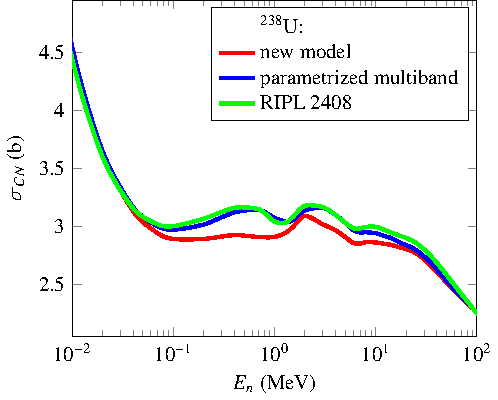
\includegraphics[width=0.7\textwidth]{images/fig1a.pdf}\\
\caption{Подпись к рисунку. Дополнительная информация}
\label{app:fig}
\end{center}
\end{figure}

дйфдфд \cite{myarticle,myrussianarticle,myproc,mybook}           % Глава 4
\include{Dissertation/conclusion}      % Заключение
\include{Dissertation/acronyms}        % Список сокращений и условных обозначений
\include{Dissertation/dictionary}      % Словарь терминов
\include{Dissertation/references}      % Список литературы
\include{Dissertation/lists}           % Списки таблиц и изображений (иллюстративный материал)

\setcounter{totalchapter}{\value{chapter}} % Подсчёт количества глав

%%% Настройки для приложений
\appendix
% Оформление заголовков приложений ближе к ГОСТ:
\setlength{\midchapskip}{20pt}
\renewcommand*{\afterchapternum}{\par\nobreak\vskip \midchapskip}
\renewcommand\thechapter{\Asbuk{chapter}} % Чтобы приложения русскими буквами нумеровались

\include{Dissertation/appendix}        % Приложения

\setcounter{totalappendix}{\value{chapter}} % Подсчёт количества приложений

\end{document}
